%!TEX root = ../../main.tex
\section{2D X-ray beam profile measurements}
\label{sec:2D X-ray beam profile measurements}
The previous section presented work on beam processing performed on measurements of the beam profile obtained from 1D aperture scans.
In this section, the analysis is described of measurements of the X-ray beam profile carried out at PETRA III synchrotron, beamline P14, Hamburg, as detailed in section \ref{sub:Data Collection and Dose Calculation}.
Specifically, the measurement was made using a scintillator combined with an Allied Vision GC1350C CCD camera, which resulted in a 2D image of the X-ray beam.
The processing of these images presents different challenges to those that arise from 1D aperture scan measurements.

The 2D image of the X-ray beam profile was exported as a portable graymap (pgm) file where each pixel contains an integer value between 0 and 255 inclusive (Figure~\ref{fig: Hamburg beam PGM}).
These values were determined by the strength of the signal from the scintillator.
To spatially resolve the flux over the beam image, RADDOSE-3D multiplied each pixel value by the ratio of the total absolute flux with the total sum of the pixel values multiplied by the area of a pixel.
This means that the pixel values can be regarded as weights that correspond to the relative photon flux at that spatial position.
In general the pgm file will always contain non-zero values that correspond to background signal.
This can be seen in Figures~\ref{fig:Hamburg beamslice} and \ref{fig:Hamburg beamslice horizontal} where the pixel values never decay to zero at any point in the slices through the beam.
RADDOSE-3D interpreted these non-zero values as beam intensity, so some of the flux that should be in the beam was instead allocated to the background pixels, which resulted in an underestimate of the absorbed dose in the crystal.
Therefore it was important to identify the background and remove it from the file before the dose simulation was performed.
Several methods for removing the background were explored and the results were compared to observe the effects on the RADDOSE-3D simulations.

\subsection{PGM file preprocessing}
\label{sub:PGM file preprocessing}

\subsubsection{Original beam profile}
\label{subs:Original beam profile}
The first profile that will be considered is the original pgm file. No preprocessing is performed on the file so that the results from other processed beams can be compared with the unprocessed case. Figure \ref{figallbeams1} shows the profile of this raw beam.

\subsubsection{Deconvolution of beam profile}
\label{subs:Deconvolution of beam profile}
The beam profile measured with the scintillator and CCD camera as described in section \ref{sub:Data Collection and Dose Calculation} can smear as a result of charge diffusion into adjacent pixels due to CCD pixel subvariations.
This response is known as the point spread function (PSF).
Thus the image formed in the pgm file is a convolution of the actual X-ray beam profile and the PSF.
To deconvolve the beam image, the following procedure was undertaken:
\begin{enumerate}
\item An initial blind deconvolution (using the MATLAB \verb+deconvblind+ function) was performed to determine an estimate of the PSF (Figure \ref{figpsf}). The blind deconvolution requires an initial guess for the PSF, but the PSF restoration in the blind deconvolution is heavily affected by the grid size of the PSF rather than the values of the grid elements. With no knowledge of the PSF (or of the signal to noise power spectrum) an initial guess for the PSF was made as a 7 $\times$ 7 grid of 1's.
\item The restored PSF was then modelled using a Laplacian function of the form
\begin{equation}
f_{lap} = \exp \left(-\f{|x| + |y|}{b}\right)
\label{eqlap}
\end{equation}
where $b$ is a parameter whose value is to be determined (Figure \ref{figmodelpsf}). The Laplacian function was chosen because it modelled the shape of the recovered PSF function very well.
\begin{figure}
        \centering
        \begin{subfigure}[b]{0.9\textwidth}
                \centering
                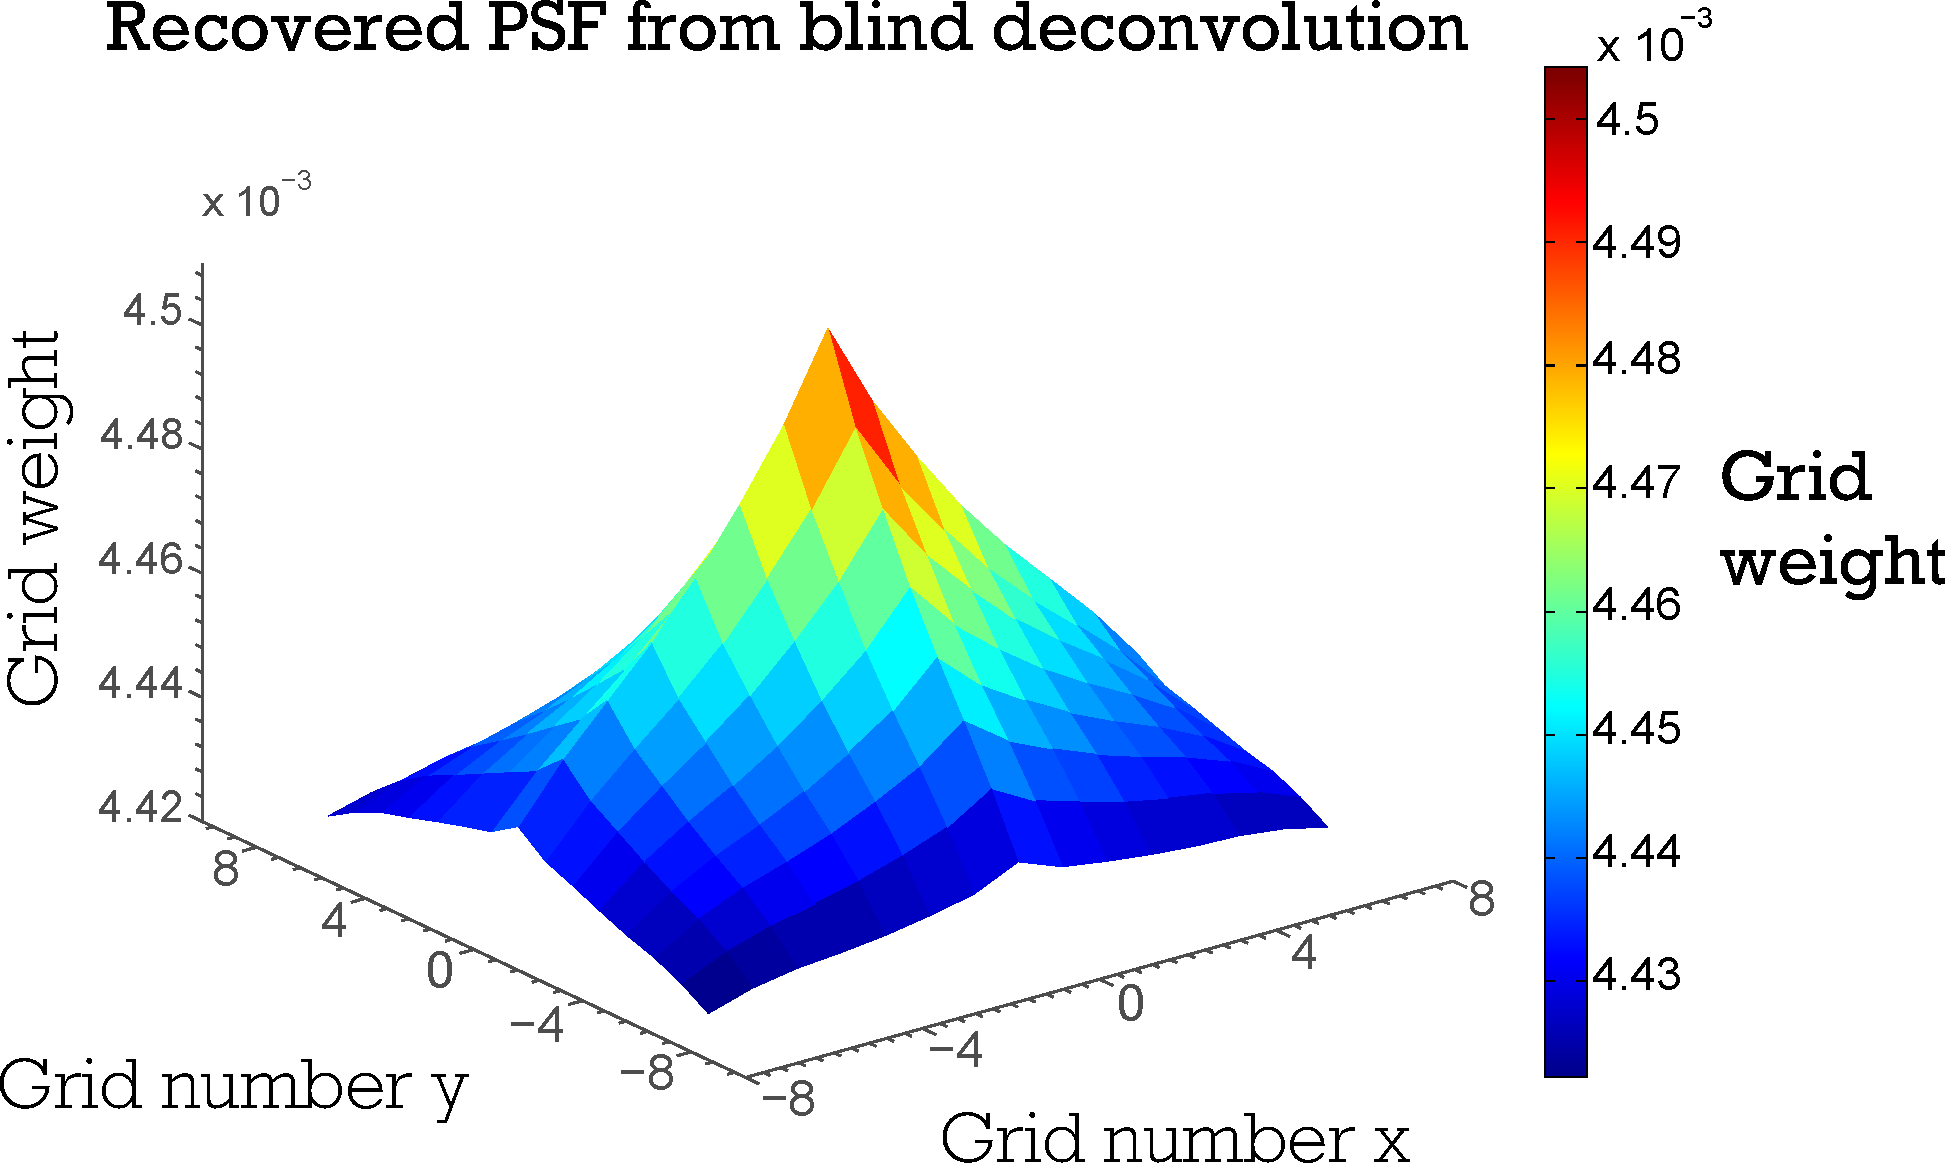
\includegraphics[width=\textwidth]{figures/beam/Initial_psf.pdf}
                \caption{}
                \label{figpsf}
        \end{subfigure}
				\\
        \begin{subfigure}[b]{0.9\textwidth}
                \centering
                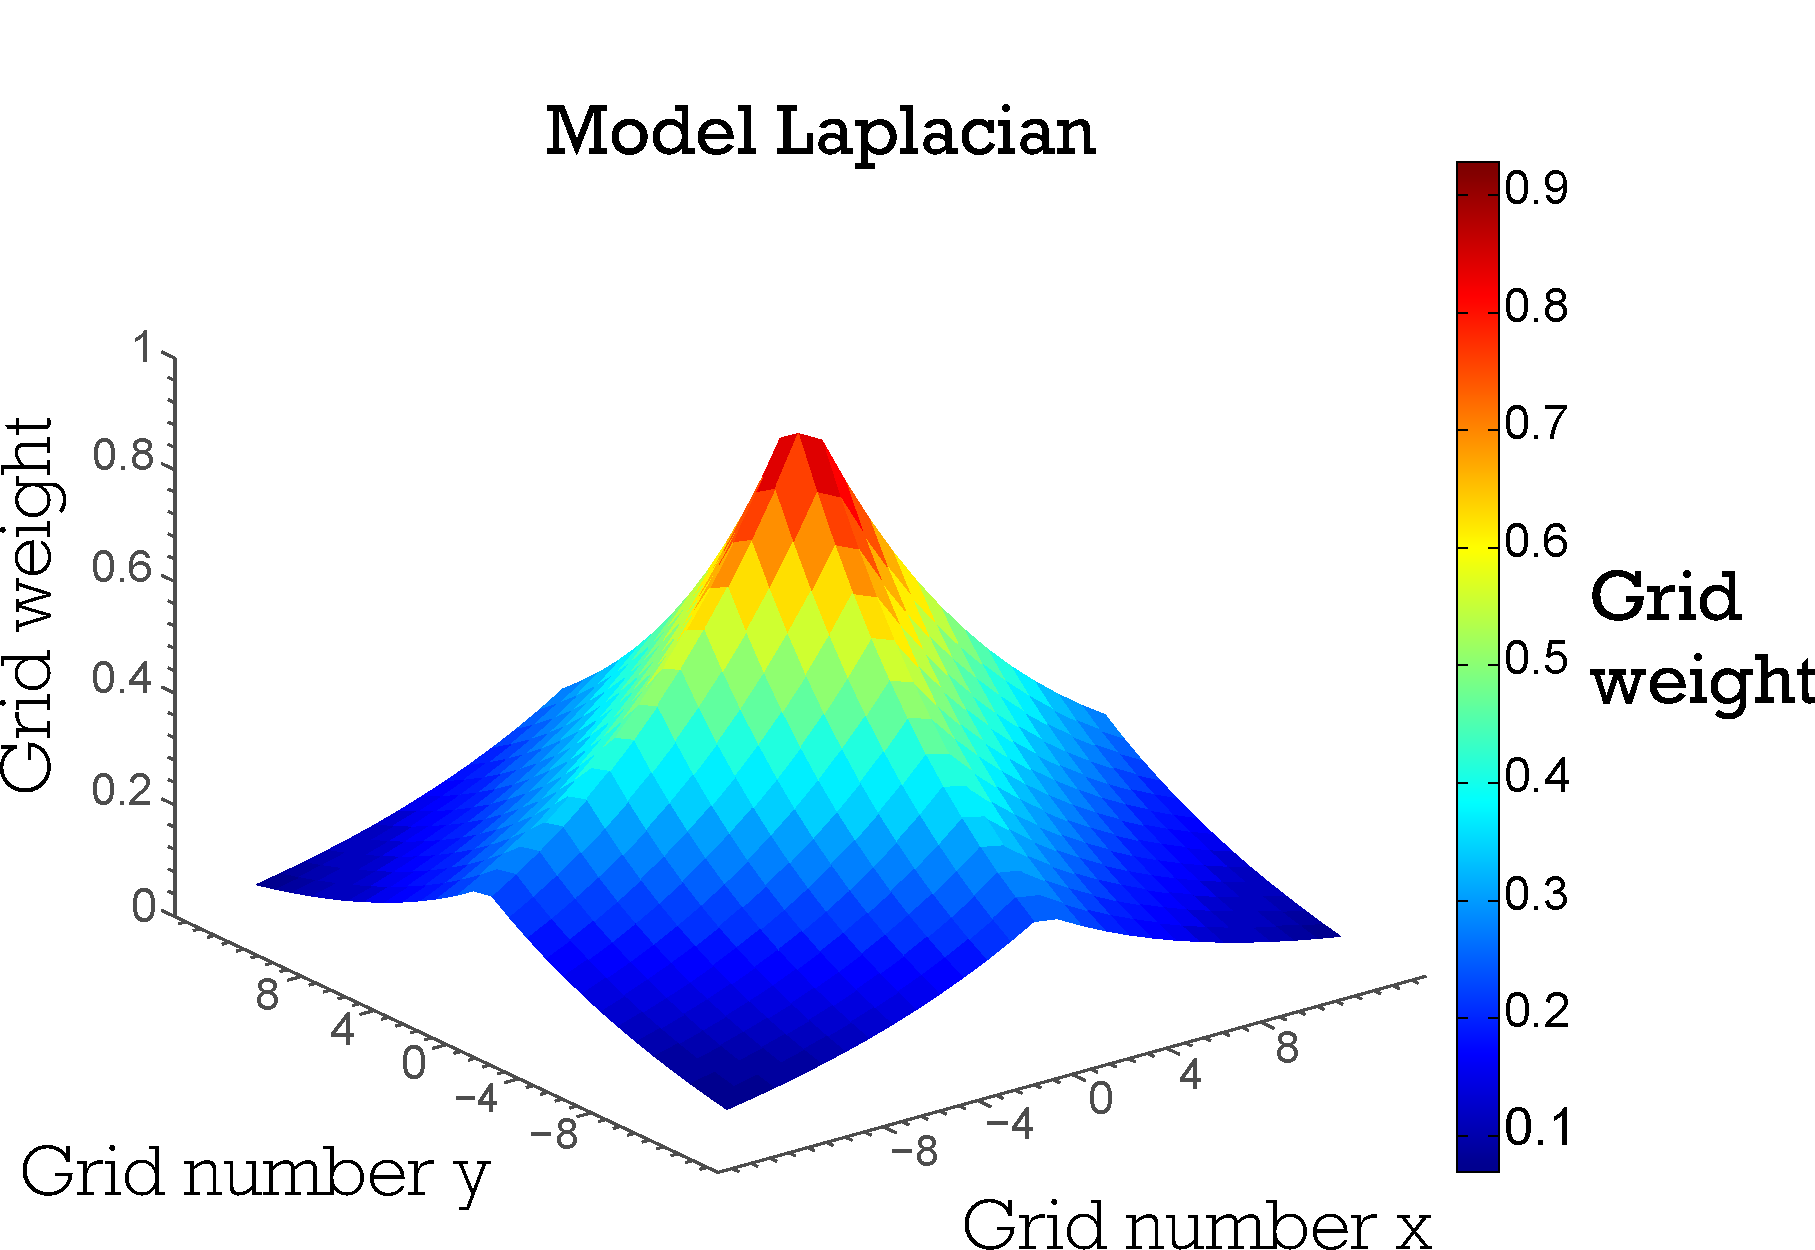
\includegraphics[width=\textwidth]{figures/beam/model_psf.pdf}
                \caption{}
                \label{figmodelpsf}
        \end{subfigure}
        \caption[Modelling of the point spread function.]{(a) PSF recovered from performing a blind deconvolution. (b) Laplacian function of the form given in equation (\ref{eqlap}) with a 7 $\times$ 7 grid and $b =$ 10.}
        \label{figpsfs}
\end{figure}
\item The pgm file was then segmented using the MATLAB \verb+activecontour+ function, which uses the Chan and Vese region based energy model \cite{chan2001}, to find the spatial area of the beam.
Additionally the centroid of the resulting image (the centre of the beam) was determined (Figure \ref{figcentroid}).
\item A rectangle that bounded the beam (inner red rectangle in Figure \ref{figbounds}) was chosen as 145$\, \mu m \times$ 140$\, \mu m$ because this contained the beam whilst allowing a buffer for beam area that may have been missed by the segmentation algorithm.
These dimensions were stored.
\begin{figure}
        \centering
        \begin{subfigure}[b]{0.9\textwidth}
                \centering
                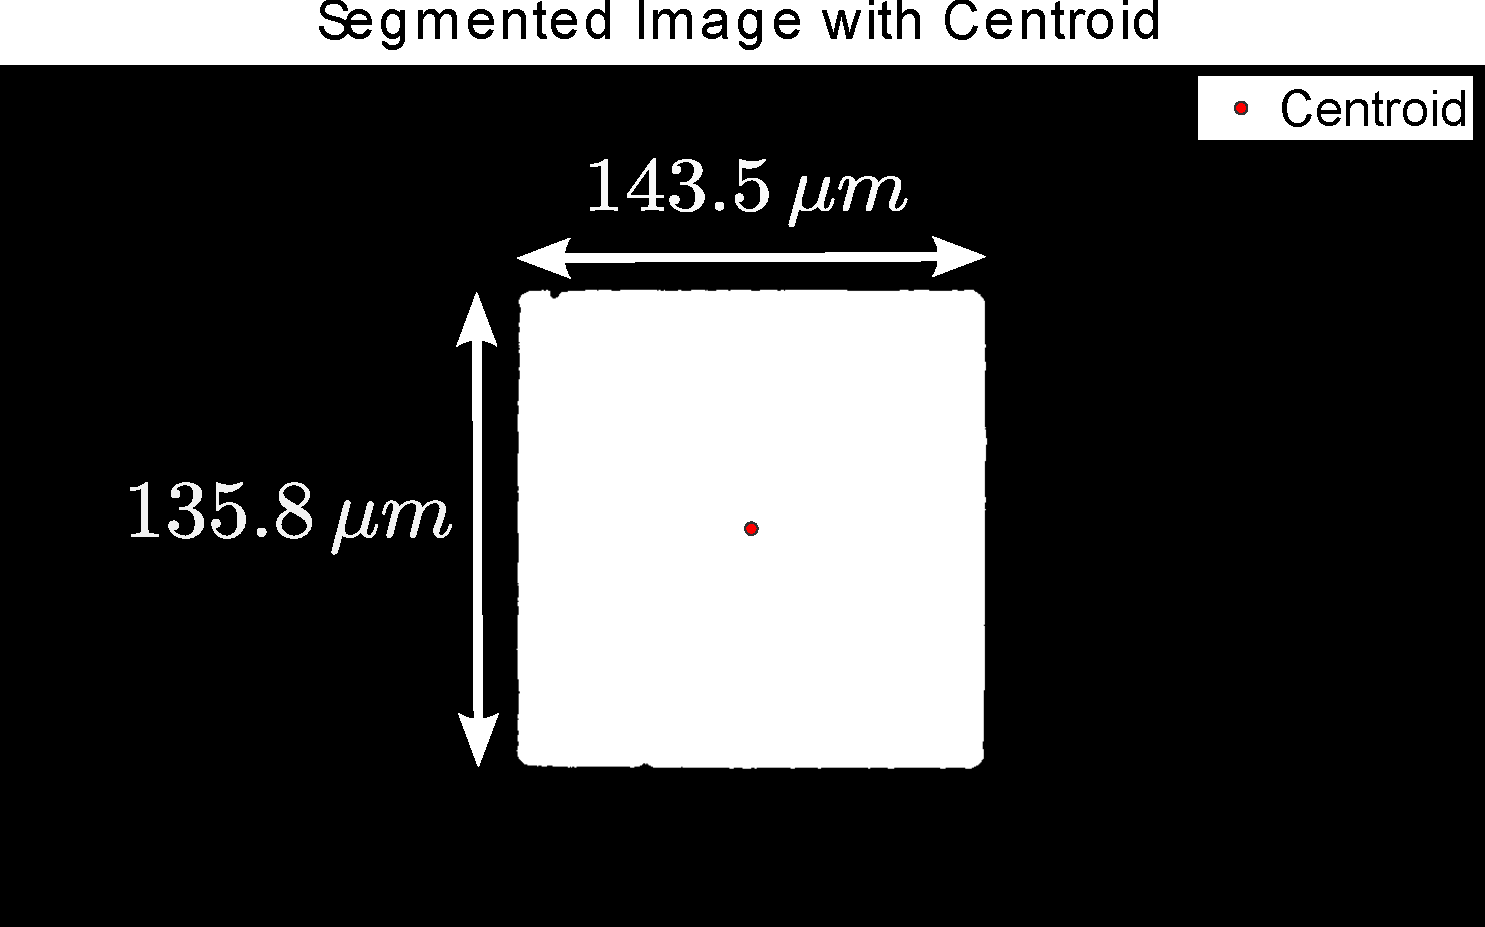
\includegraphics[width=\textwidth]{figures/beam/seg_image.pdf}
                \caption{}
                \label{figcentroid}
        \end{subfigure}
				\\
        \begin{subfigure}[b]{0.9\textwidth}
                \centering
                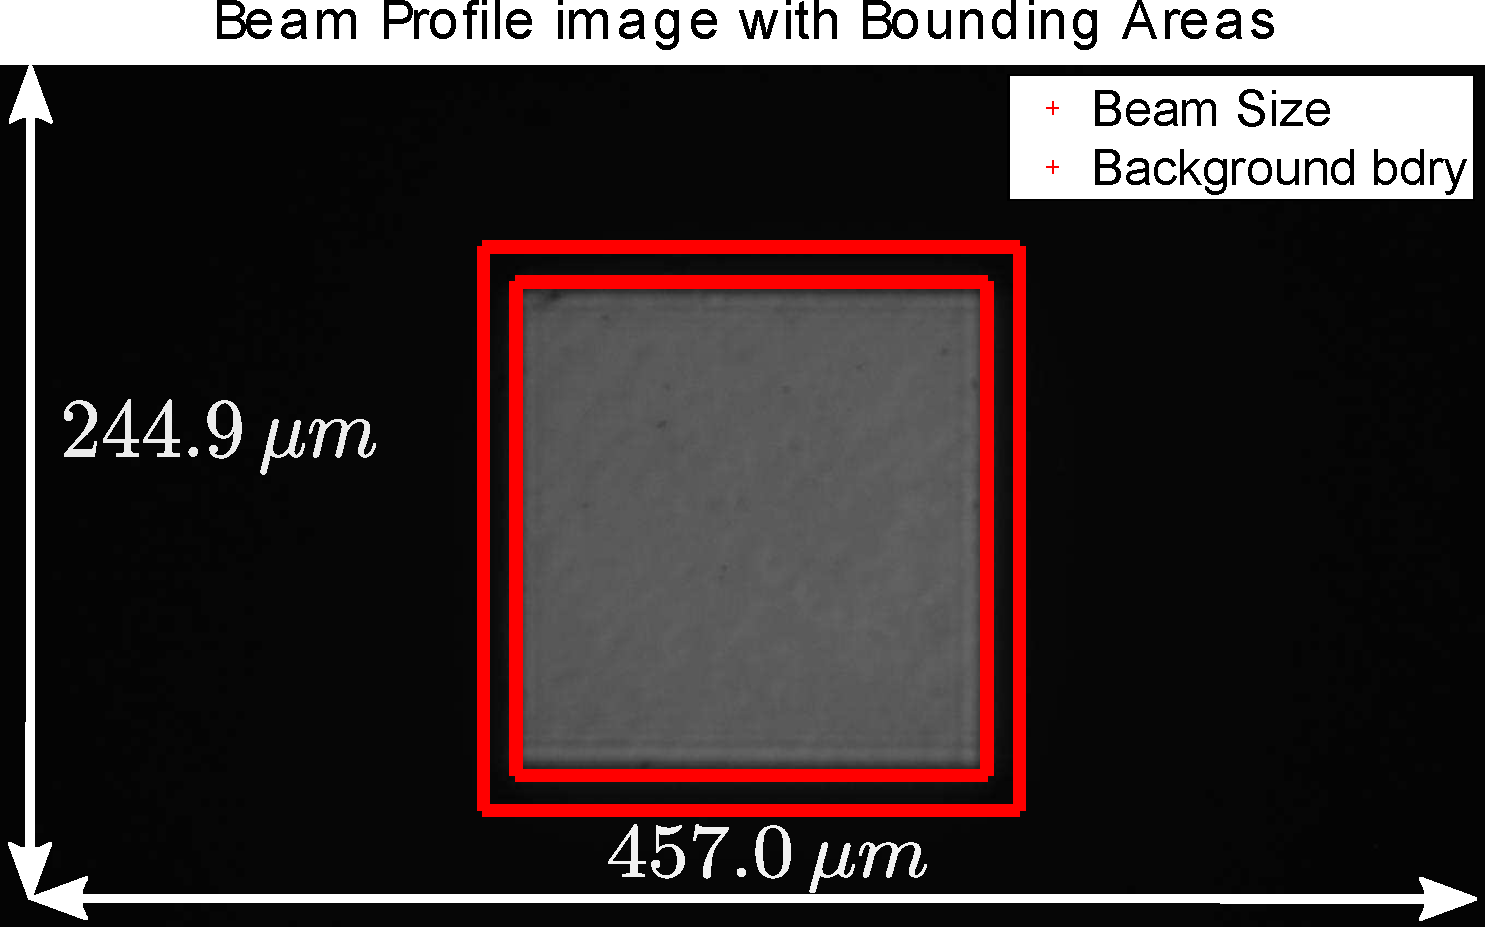
\includegraphics[width=\textwidth]{figures/beam/bounding_areas2.pdf}
                \caption{}
                \label{figbounds}
        \end{subfigure}
        \caption[Beam image segmentation and beam boundaries.]{(a) Segmented image of the beam with its centroid marked as a red circle in the middle.
        (b) Beam image with the centroid and two bounding boxes overlaid.
        The inner box is an estimate of the beam size with dimensions 145$\, \mu m \times$ 140$\, \mu m$.
        These dimensions were chosen according to the coverage of the beam area in the image as opposed to the size of the aperture from the slit separation (slits were set at 140$\,\mu m \times$ 140$\,\mu m$).
        The outer box is the boundary,170$\, \mu m \times$ 170$\, \mu m$, where the pixels outside the box are considered part of the background (section \ref{secthresh}).}
        \label{figimagemanip}
\end{figure}
\item The (square) grid size for the PSF, $b$ in equation \ref{eqlap} and the rectangular dimensions were then used as inputs for an objective function in a minimisation process to determine optimal values for these parameters. The objective function was constructed as follows:
\begin{itemize}
\item A perfect (hypothetical) top hat beam was created inside the inner box (Figure \ref{figbounds}).
\item The Laplacian PSF was created using the grid size and $b$.
\item The top hat beam was convolved with the PSF to create a theoretical (convolved) beam image.
\item the positions of zero pixel values from the theoretical beam image were also set to zero in the original beam image.
\item The height of the theoretical beam image was adjusted by a factor of the mean of the original beam height, divided by the modal value of the theoretical beam height (the zero pixel values were discarded for the mean and mode calculations).
This ensured that the values of the beams were on the same scale.
\item The matrix 2-norm of the difference between the original beam image with zeroed outer pixel values and the theoretical beam image was calculated and used as the output of the objective function to be minimised (the matrix 2-norm is equal to the square root of the maximum eigenvalue of the matrix multiplied by its conjugate transpose matrix).
\end{itemize}
\item Another blind deconvolution was performed as before but this time with the returned grid size from the minimisation procedure as the input.
The resulting beam profile was then returned for input into RADDOSE-3D (Figure \ref{figallbeams2}).
\end{enumerate}

\subsubsection{Removal of background using deconvolution results}
Since the rectangular dimensions of the hypothetical top-hat beam were given as outputs of the minimisation procedure, this shape can be used to distinguish between the X-ray beam and background.
The two beams described above were also further manipulated by setting any values outside of the rectangle dimensions (inner box) to zero (Figures \ref{figallbeams3} and \ref{figallbeams4}).

\subsubsection{Perfect top hat beam}
A perfect top hat beam was created within the inner boundary of Figure~\ref{figbounds}  i.e. the value 100 was inserted for pixels that lay inside the inner rectangle, otherwise the pixel values were set to zero (Figure \ref{figallbeams9}).

\subsubsection{Beam thresholding}
\label{secthresh}
In his D. Phil. thesis, Dr. Oliver Zeldin preprocessed pgm files by setting a threshold value \cite{zeldin2013thesis}.
The threshold (or dark current) value was determined by taking the average of the pixel values that were ``far away'' from the main beam centre.
However, to my knowledge, there was no systematic way to determine ``far away''.
In the PETRA III MX experiment described here, the slits were adjusted to give an aperture of 140 $\times$ 140$\, \mu m^{\text{2}}$.
To determine how the choice of ``far away'' affects the threshold to be subtracted, it was decided that background would be considered as any pixel value beyond 30$\,\mu m$ away from the slit edge (Bkgd$_{\text{30}}$).
The 170 $\times$ 170$\, \mu m^{\text{2}}$ outer red box in Figure \ref{figbounds} is the Bkgd$_{\text{30}}$ boundary.
Another two beams were created assuming that the background could be considered as any pixel beyond 20$\,\mu m$ from the slit edge (Bkgd$_{\text{20}}$ with a 160 $\times$ 160$\, \mu m^{\text{2}}$ boundary) and 85$\,\mu m$ from the slit edge (Bkgd$_{\text{85}}$ with a 225 $\times$ 225$\, \mu m^{\text{2}}$ boundary).
These boundaries are shown in Figure \ref{figbackgrounds}.
\begin{figure}
	\begin{adjustwidth}{-0.75cm}{}
        \centering
        \begin{subfigure}[b]{0.45\textwidth}
                \centering
                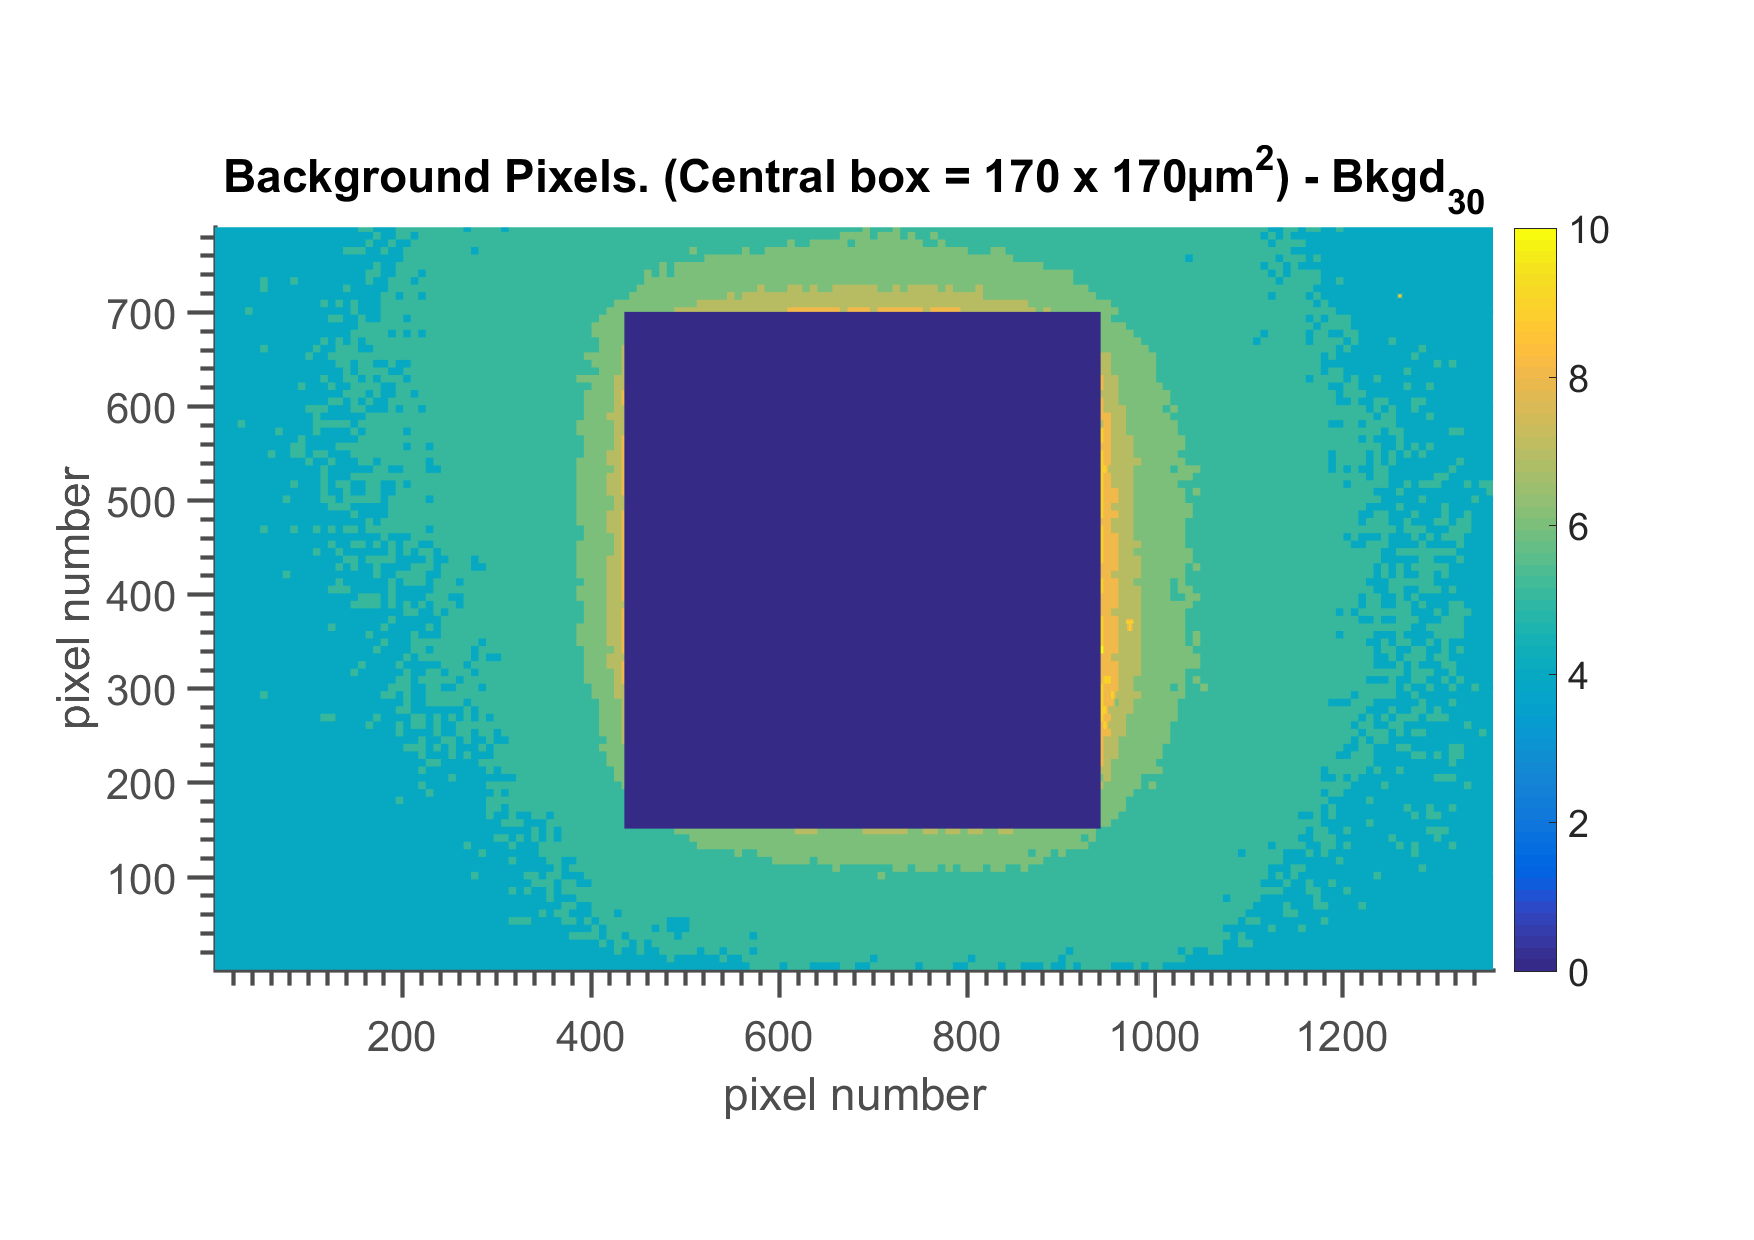
\includegraphics[width=8cm, height=8cm, angle =0]{figures/beam/figbackground170.pdf}
                \caption{}
                \label{figbackgrounds170}
        \end{subfigure}
				\qquad
        \begin{subfigure}[b]{0.45\textwidth}
                \centering
                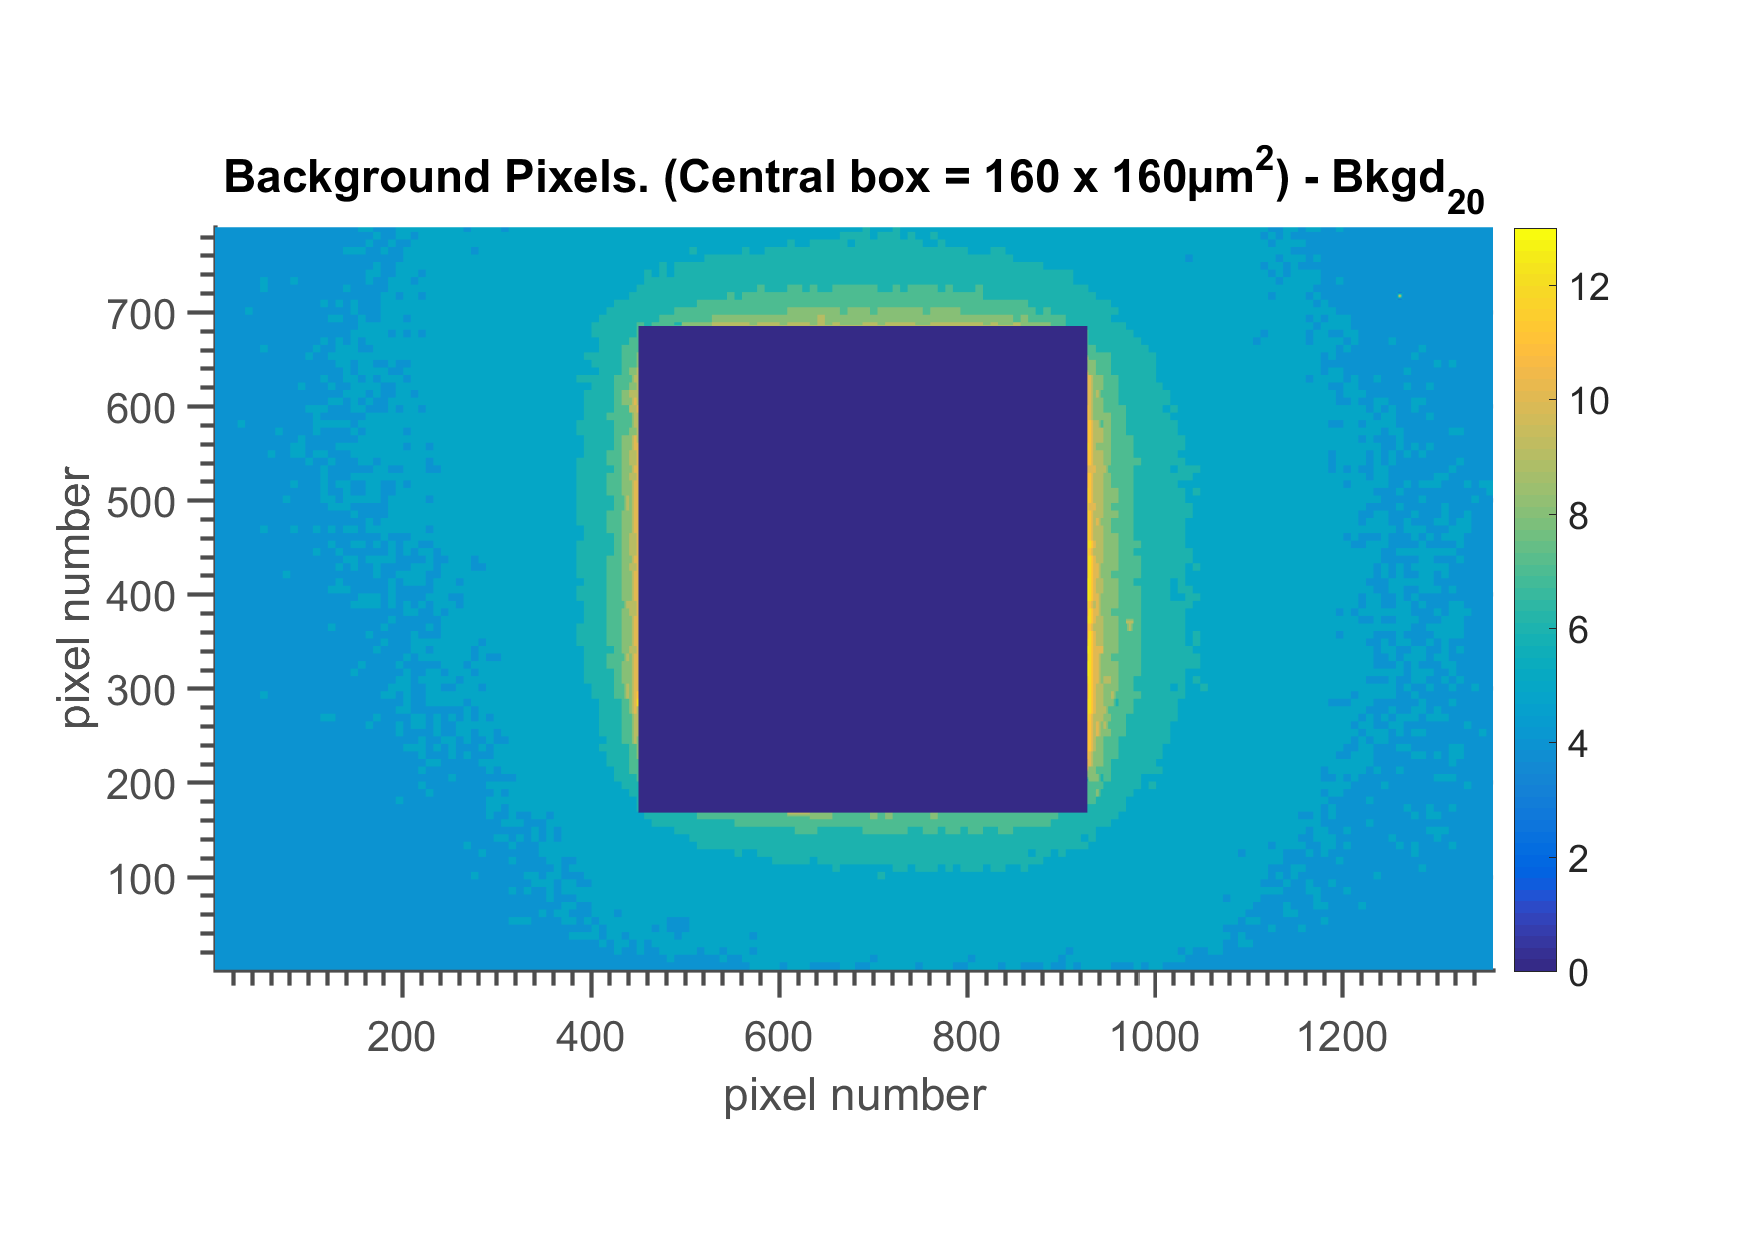
\includegraphics[width=8cm, height=8cm,, angle =0 ]{figures/beam/figbackground160.pdf}
                \caption{}
                \label{figbackgrounds160}
        \end{subfigure}
				\\
				\begin{subfigure}[b]{0.45\textwidth}
                \centering
                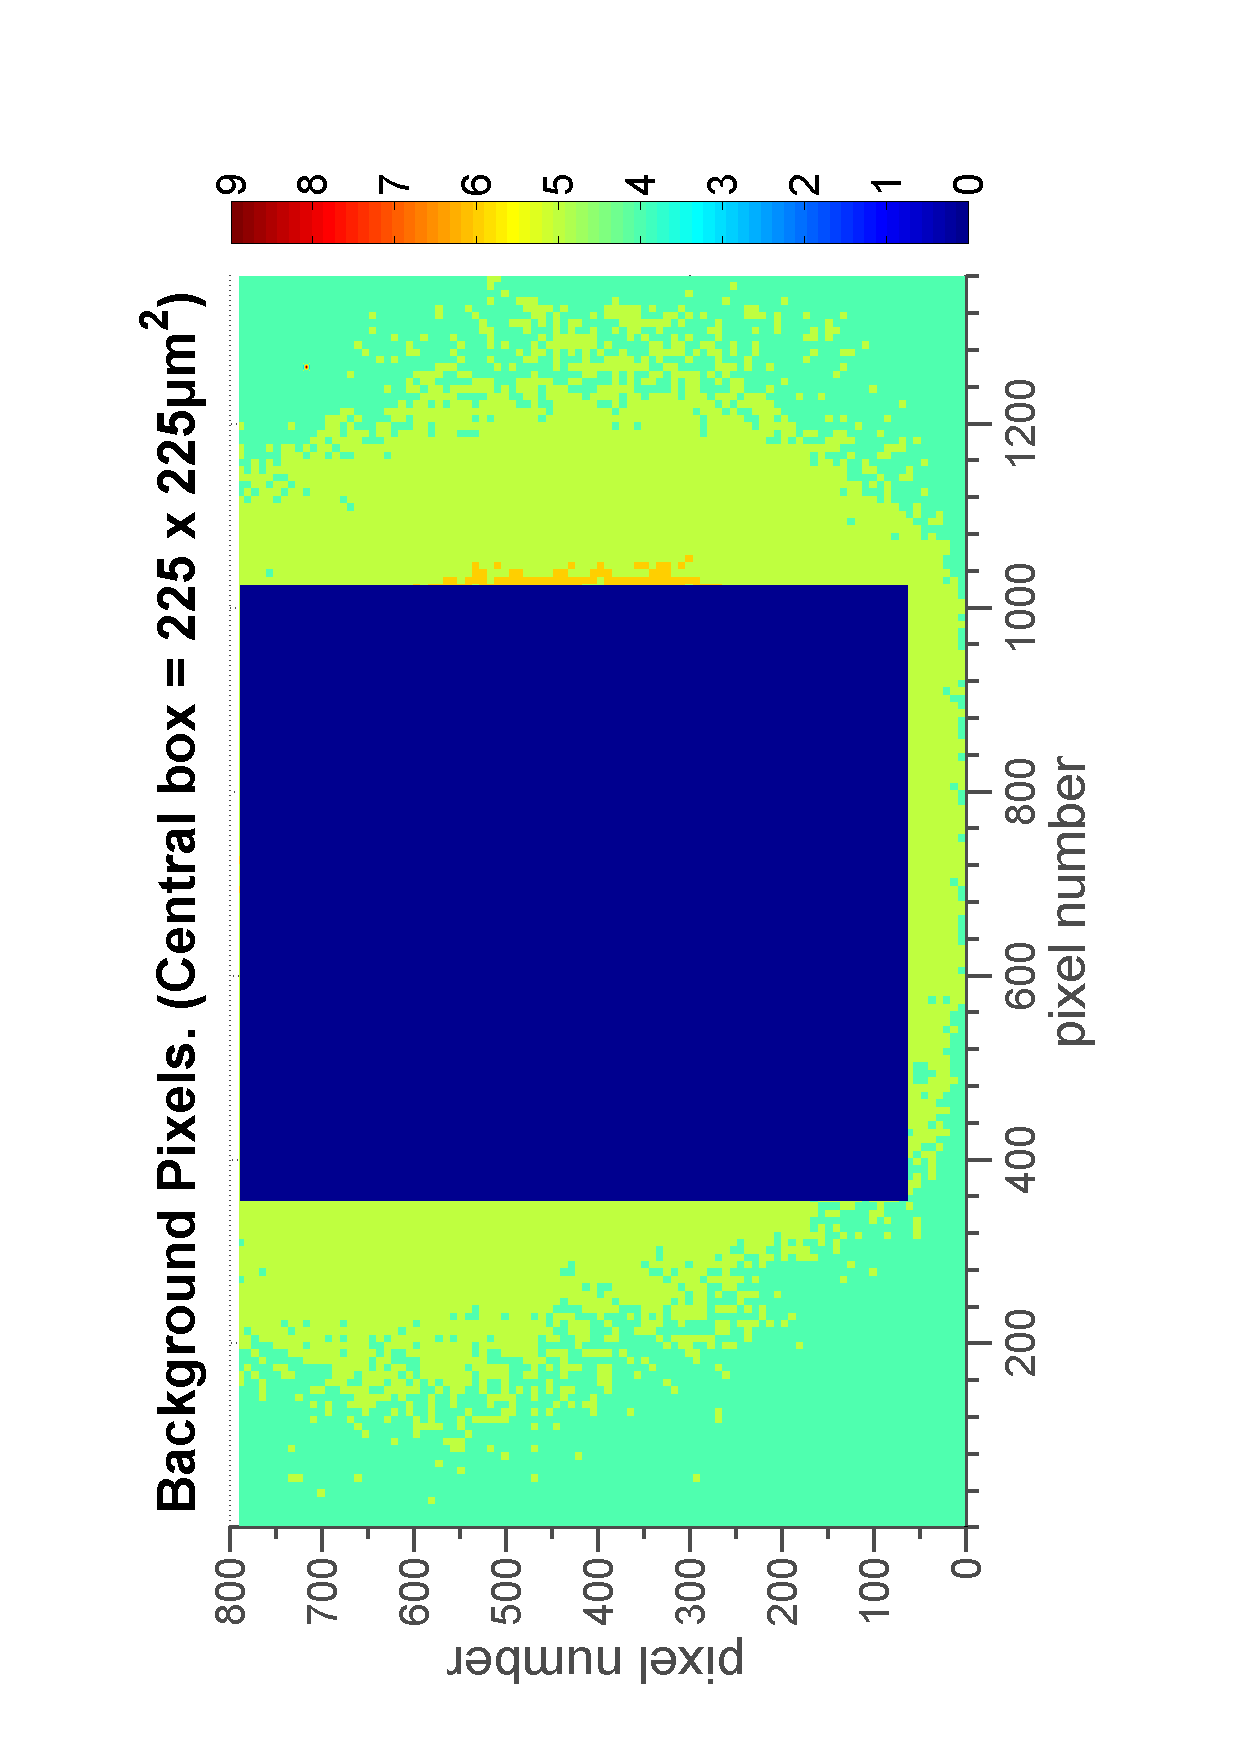
\includegraphics[width=8cm, height=8cm,, angle =0 ]{figures/beam/figbackground225.pdf}
                \caption{}
                \label{figbackgrounds225}
        \end{subfigure}
        \caption[Background pixels of the X-ray beam image.]{Background pixel values for the beam image (beam image dimensions are 457.0$\, \mu m \times$ 244.9$\, \mu m$ for all images).
        The pixel values in the central box for all images are set to zero and the mean and maximum values of the non-zero pixel values are taken for each of the backgrounds.
        (a) Bkgd$_{\text{30}}$: Rounded mean pixel value = 5, maximum pixel value = 10.
        (b) Bkgd$_{\text{20}}$: Rounded mean pixel value = 5, maximum pixel value = 13.
        (c) Bkgd$_{\text{85}}$: Rounded mean pixel value = 4, maximum pixel value = 9.}
        \label{figbackgrounds}
	\end{adjustwidth}
\end{figure}
The threshold value for subtraction was determined by taking a mean average of the background pixel values and rounding it to the nearest integer (Figures \ref{figallbeams5}, \ref{figallbeams6} and \ref{figallbeams10}). Another way to determine the background was to take the maximum value of the background values and subtract that value from every pixel in the image (Figures \ref{figallbeams7}, \ref{figallbeams8} and \ref{figallbeams11}).
\begin{figure}
        \centering
        \begin{subfigure}[b]{0.45\textwidth}
                \centering
                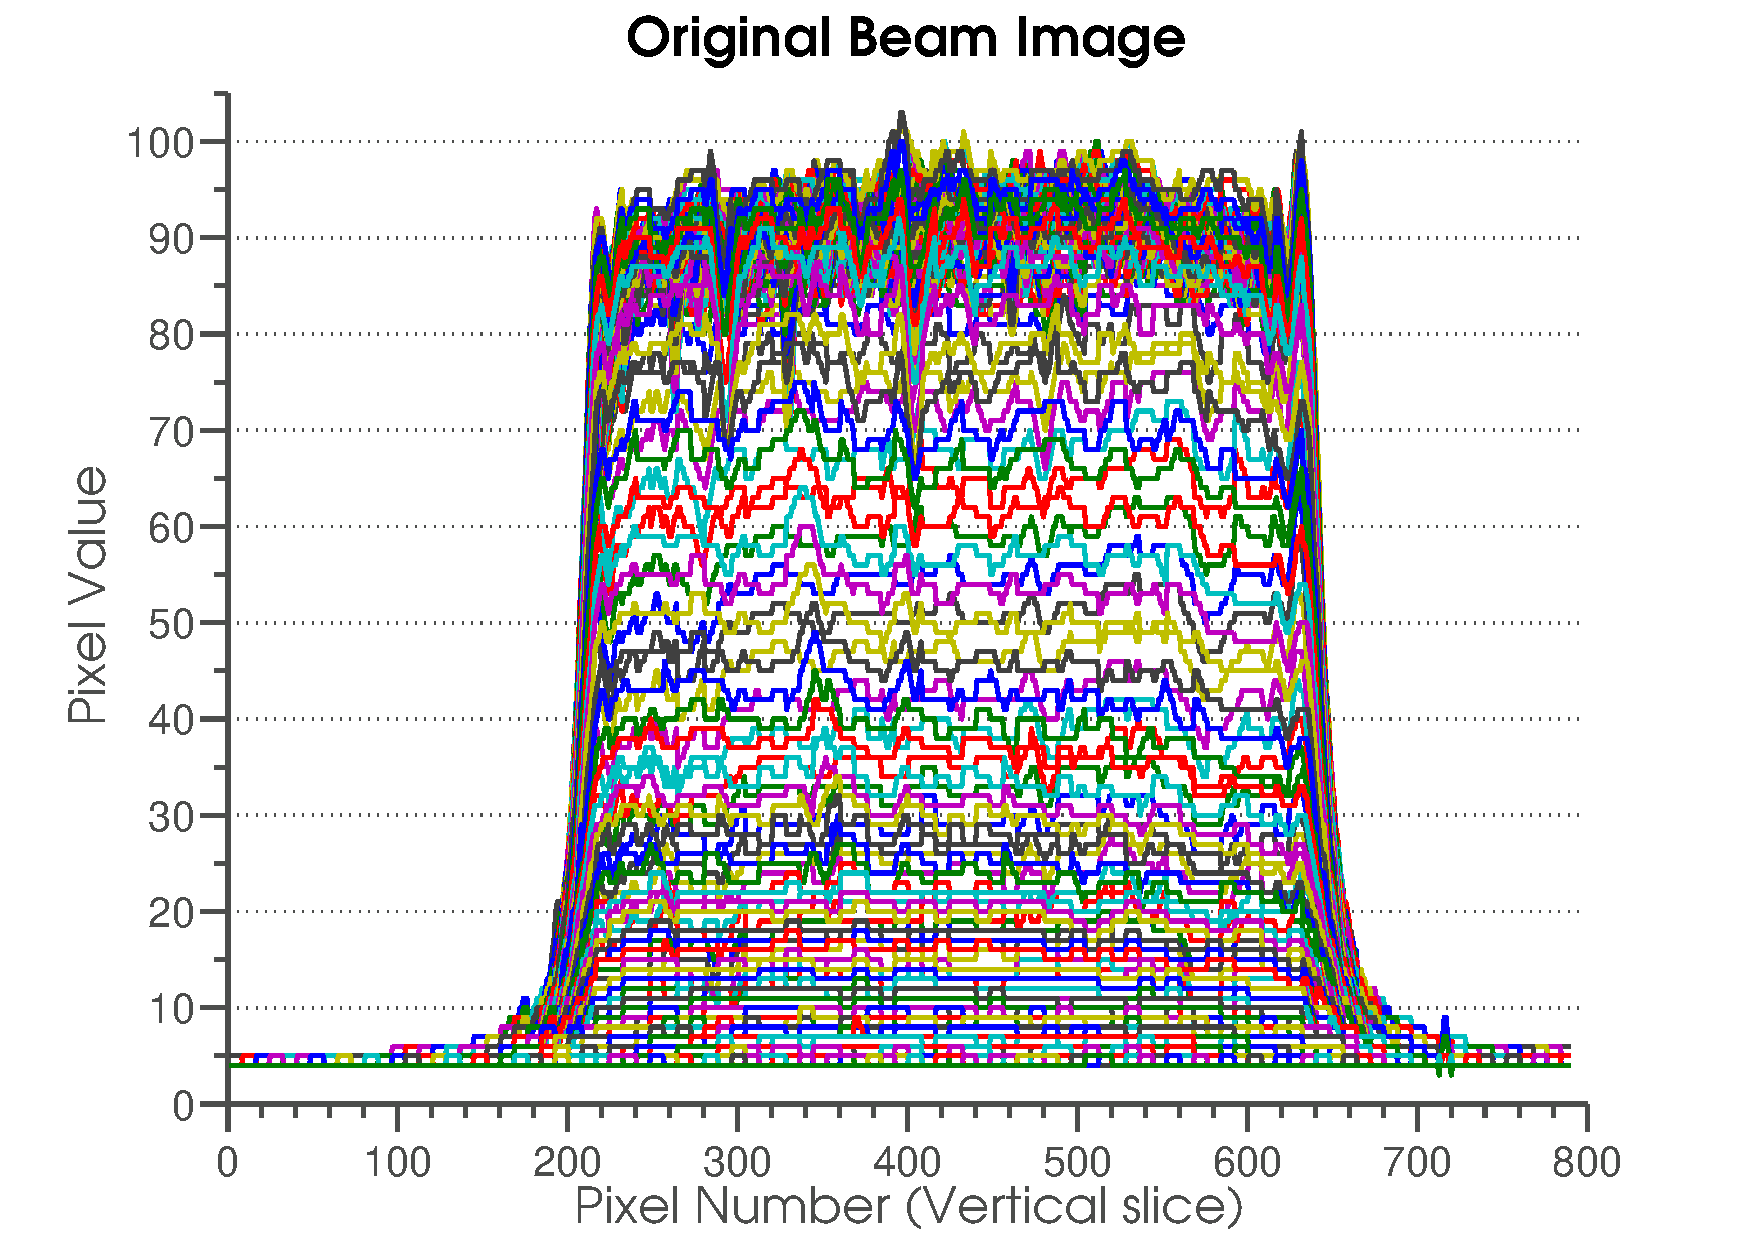
\includegraphics[width=\textwidth]{figures/beam/fig_beam_orig.pdf}
                \caption{}
                \label{figallbeams1}
        \end{subfigure}
				\qquad
        \begin{subfigure}[b]{0.45\textwidth}
                \centering
                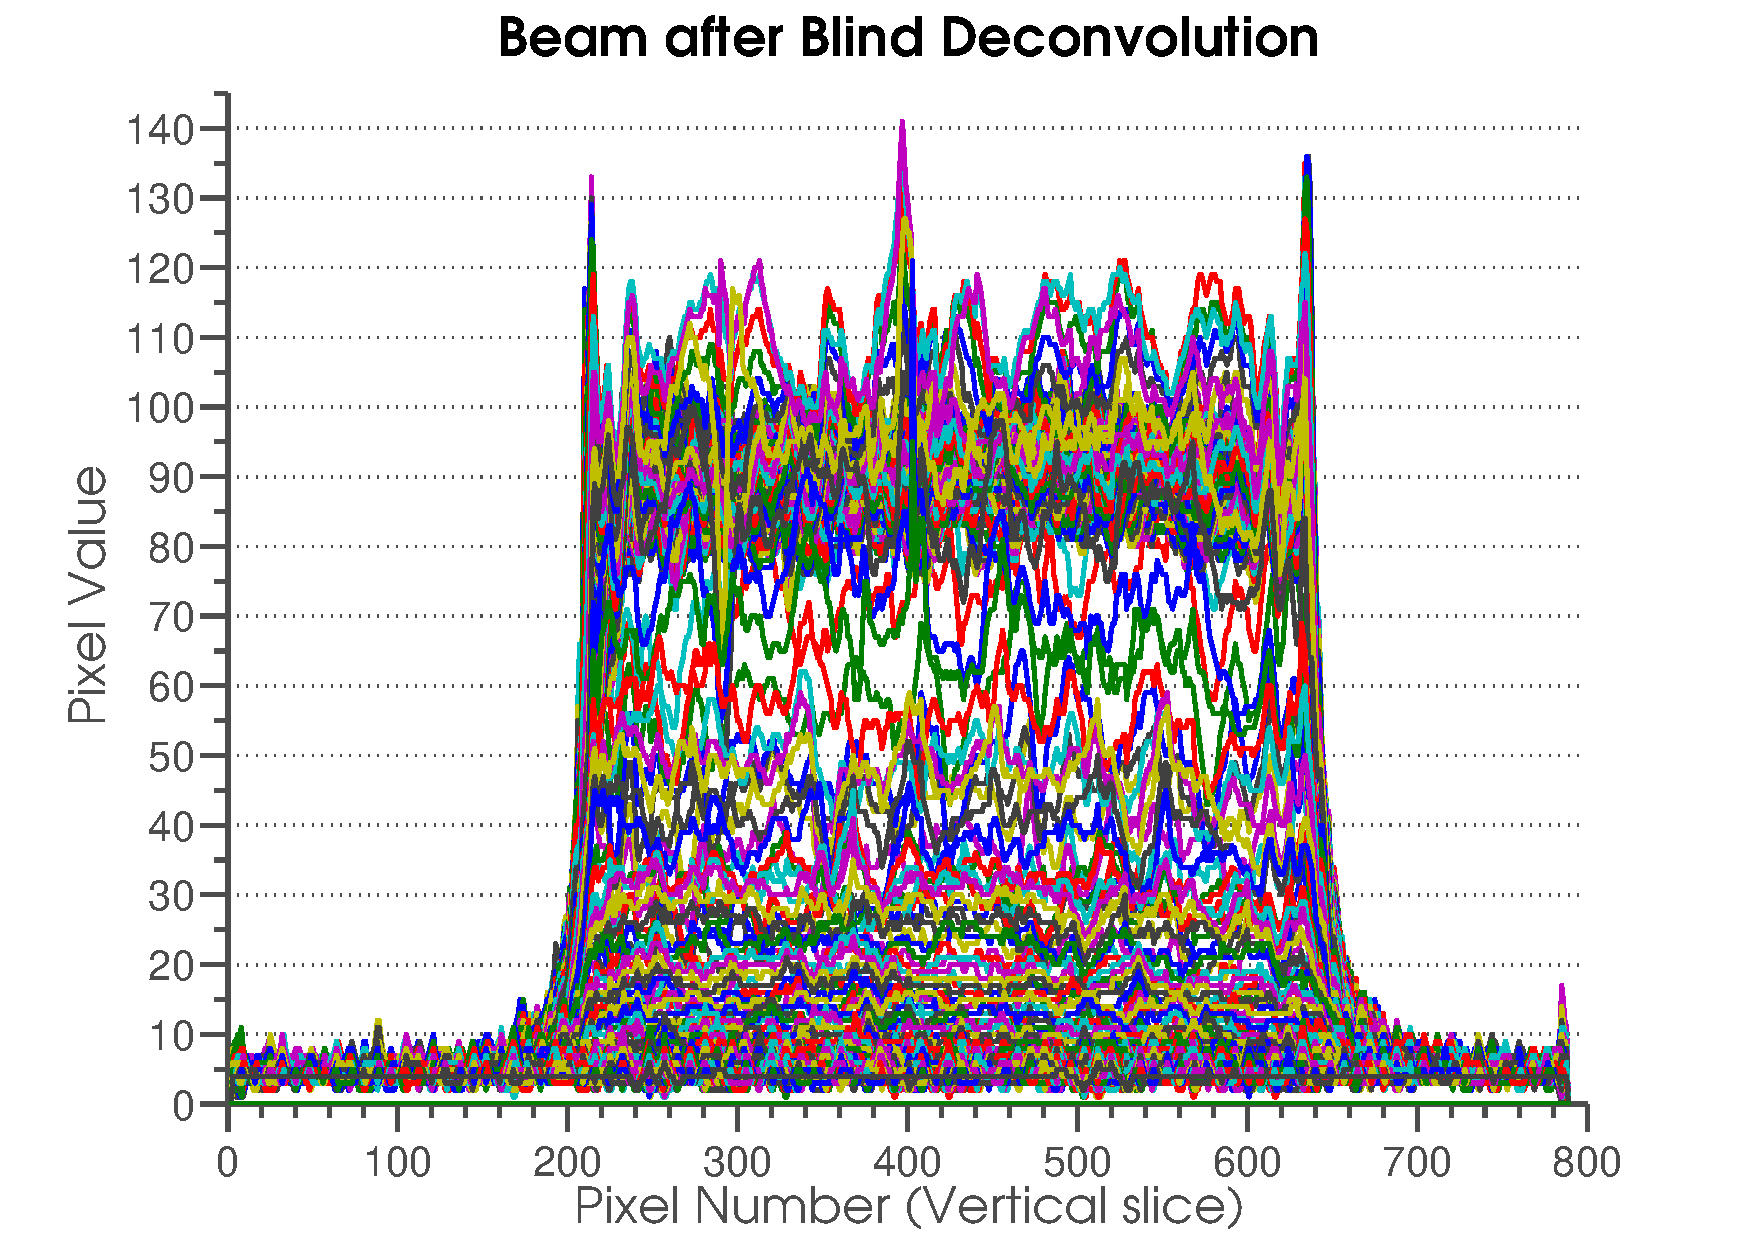
\includegraphics[width=\textwidth]{figures/beam/fig_beam_blind.pdf}
                \caption{}
                \label{figallbeams2}
        \end{subfigure}
				\\
				\begin{subfigure}[b]{0.45\textwidth}
                \centering
                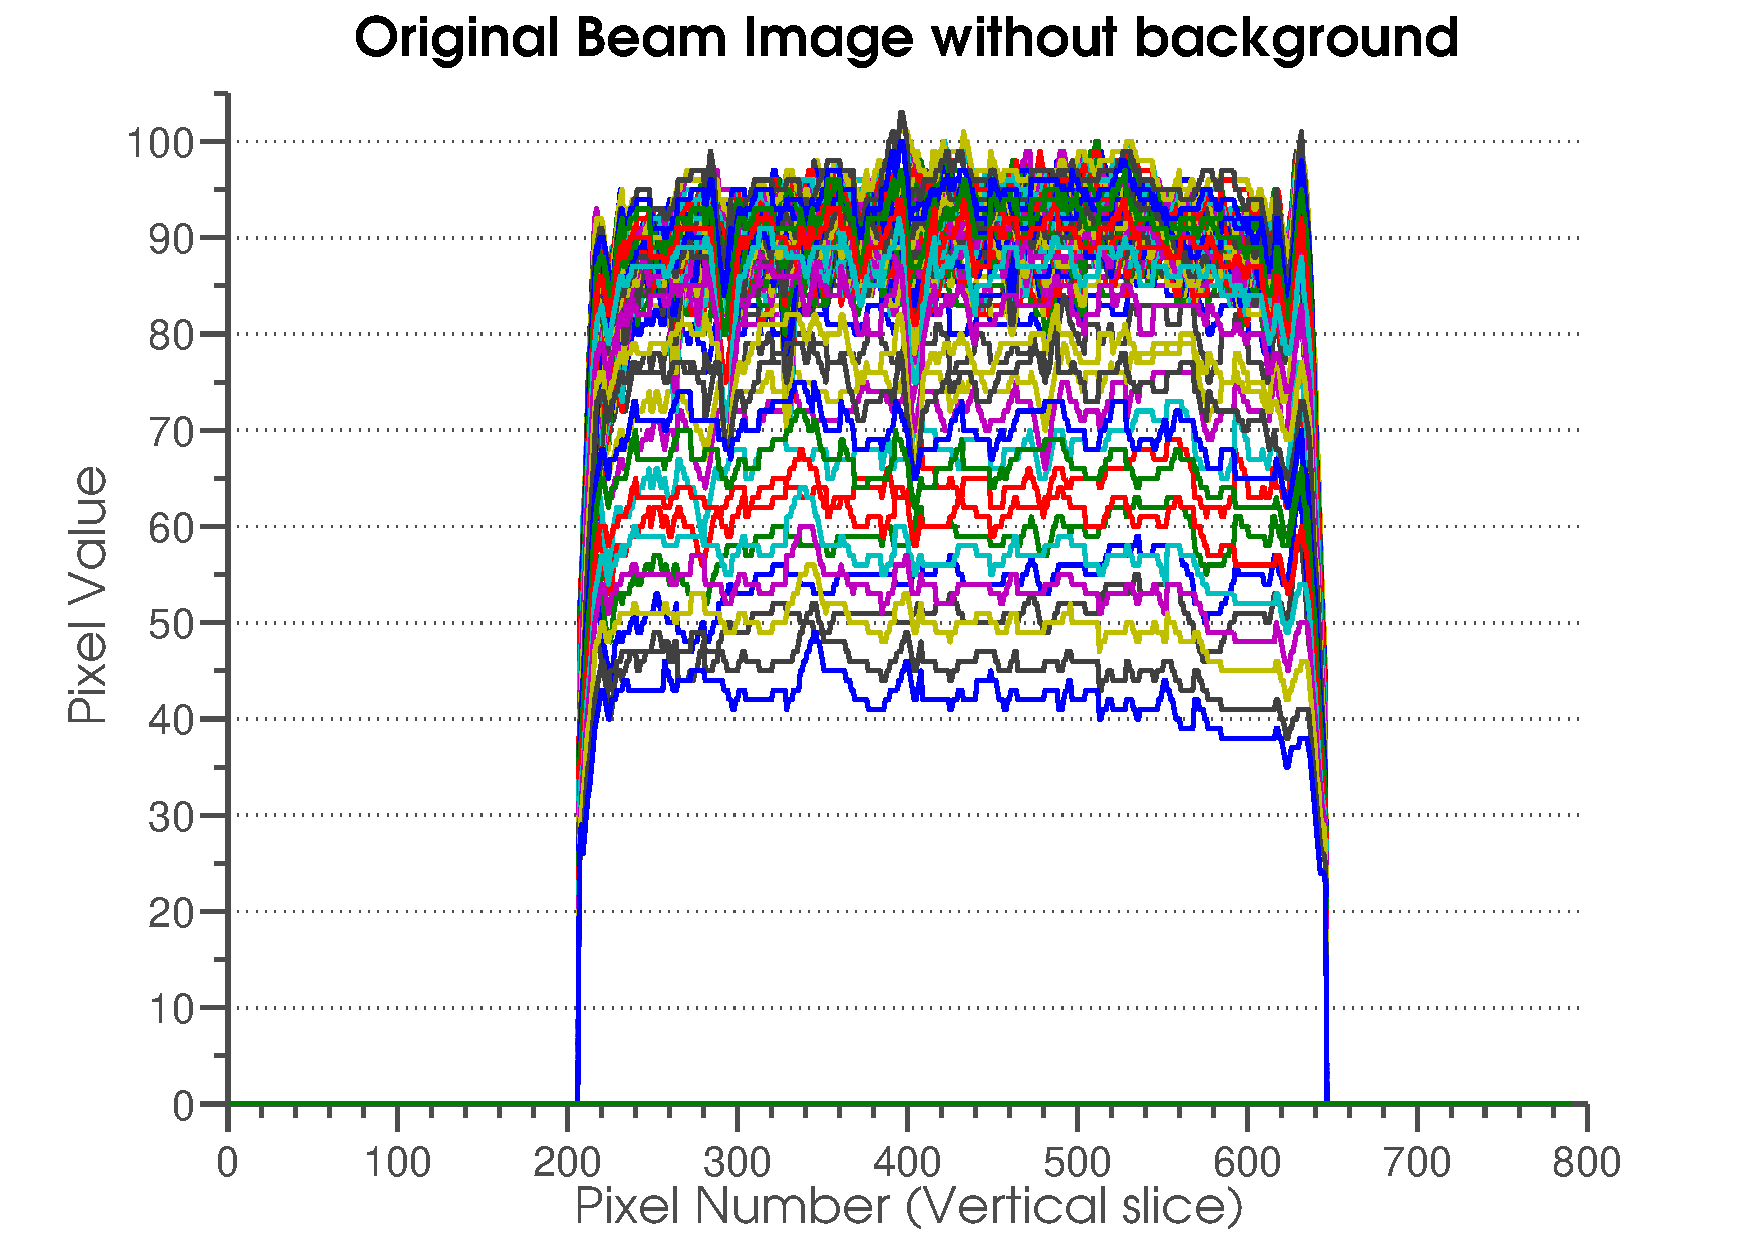
\includegraphics[width=\textwidth]{figures/beam/fig_beam_orig_cut.pdf}
                \caption{}
                \label{figallbeams3}
        \end{subfigure}
				\qquad
        \begin{subfigure}[b]{0.45\textwidth}
                \centering
                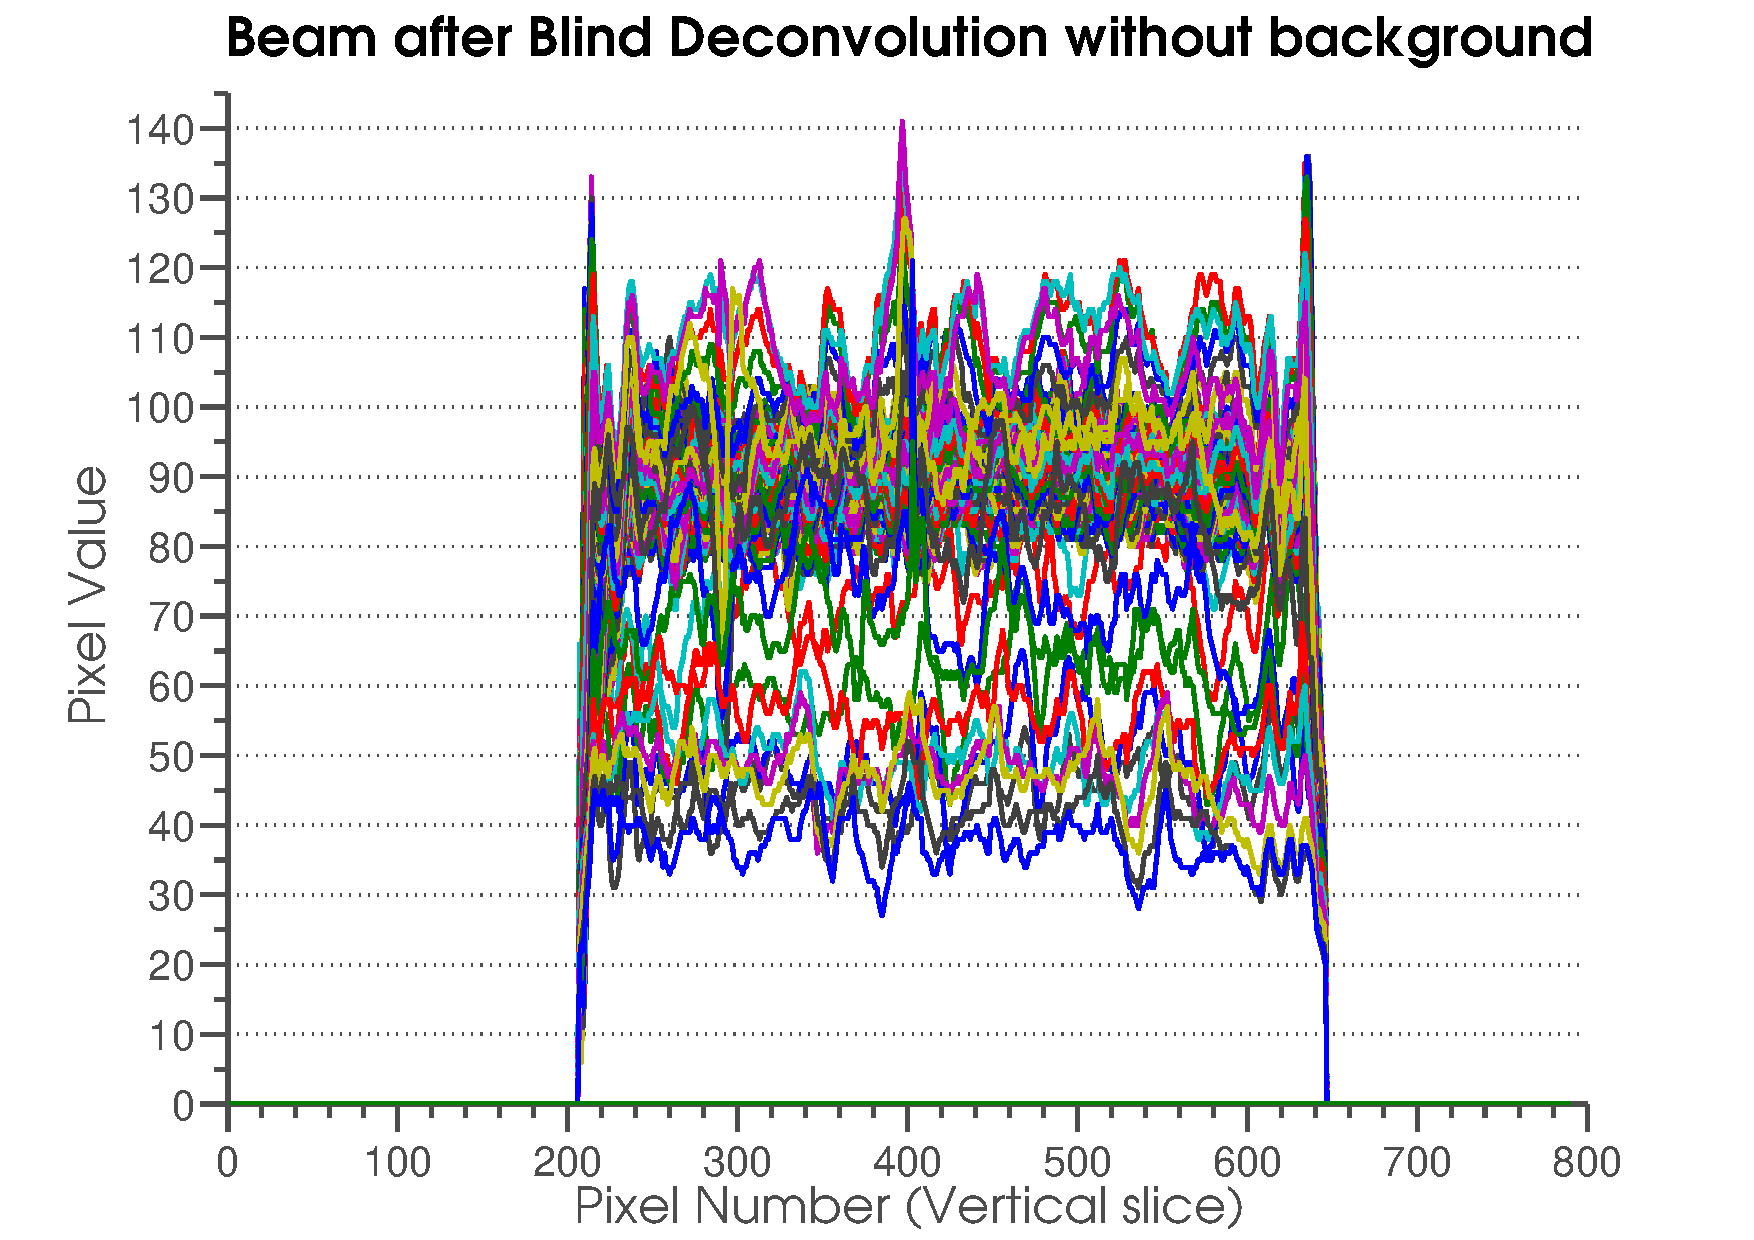
\includegraphics[width=\textwidth]{figures/beam/fig_beam_blind_cut.pdf}
                \caption{}
                \label{figallbeams4}
        \end{subfigure}
				\\
				\begin{subfigure}[b]{0.45\textwidth}
                \centering
                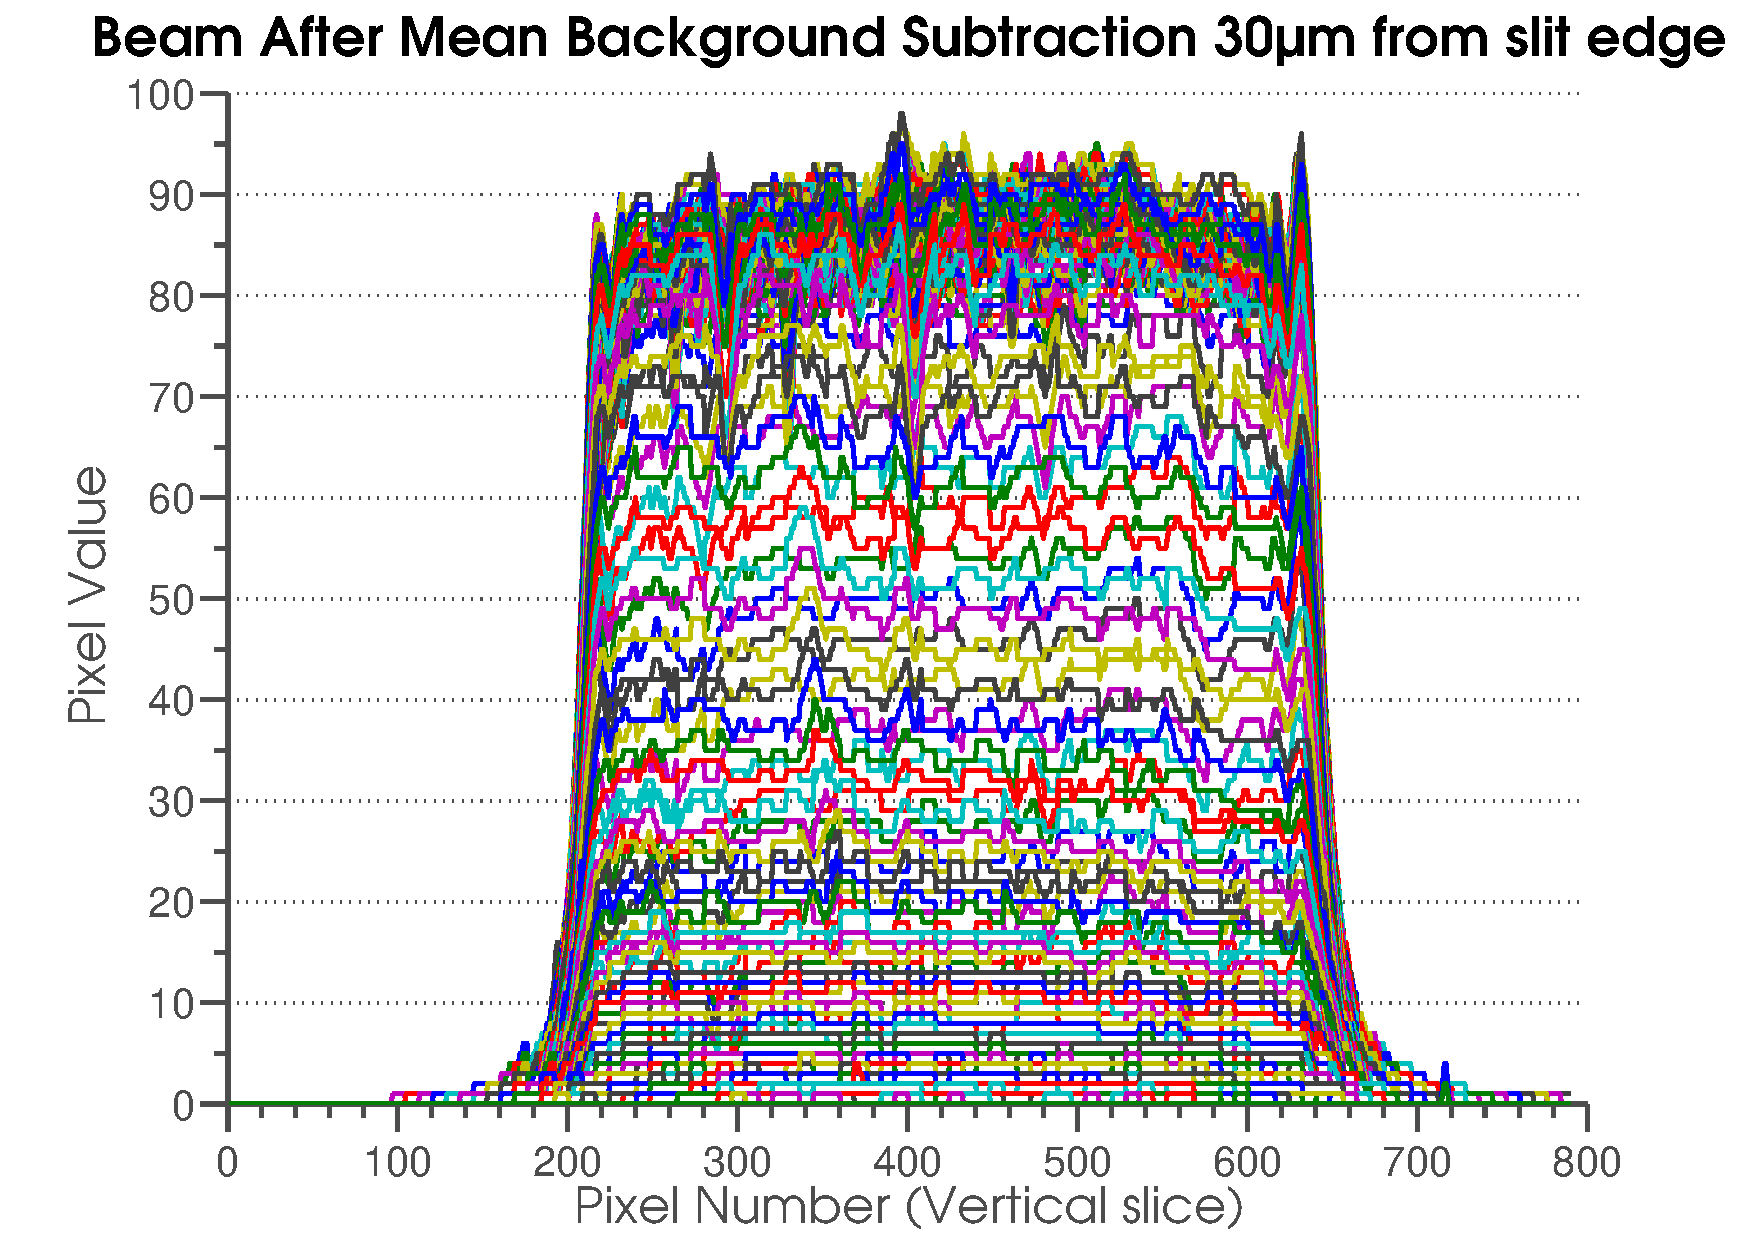
\includegraphics[width=\textwidth]{figures/beam/fig_beam_blind_thres170_mean.pdf}
                \caption{}
                \label{figallbeams5}
        \end{subfigure}
				\qquad
        \begin{subfigure}[b]{0.45\textwidth}
                \centering
                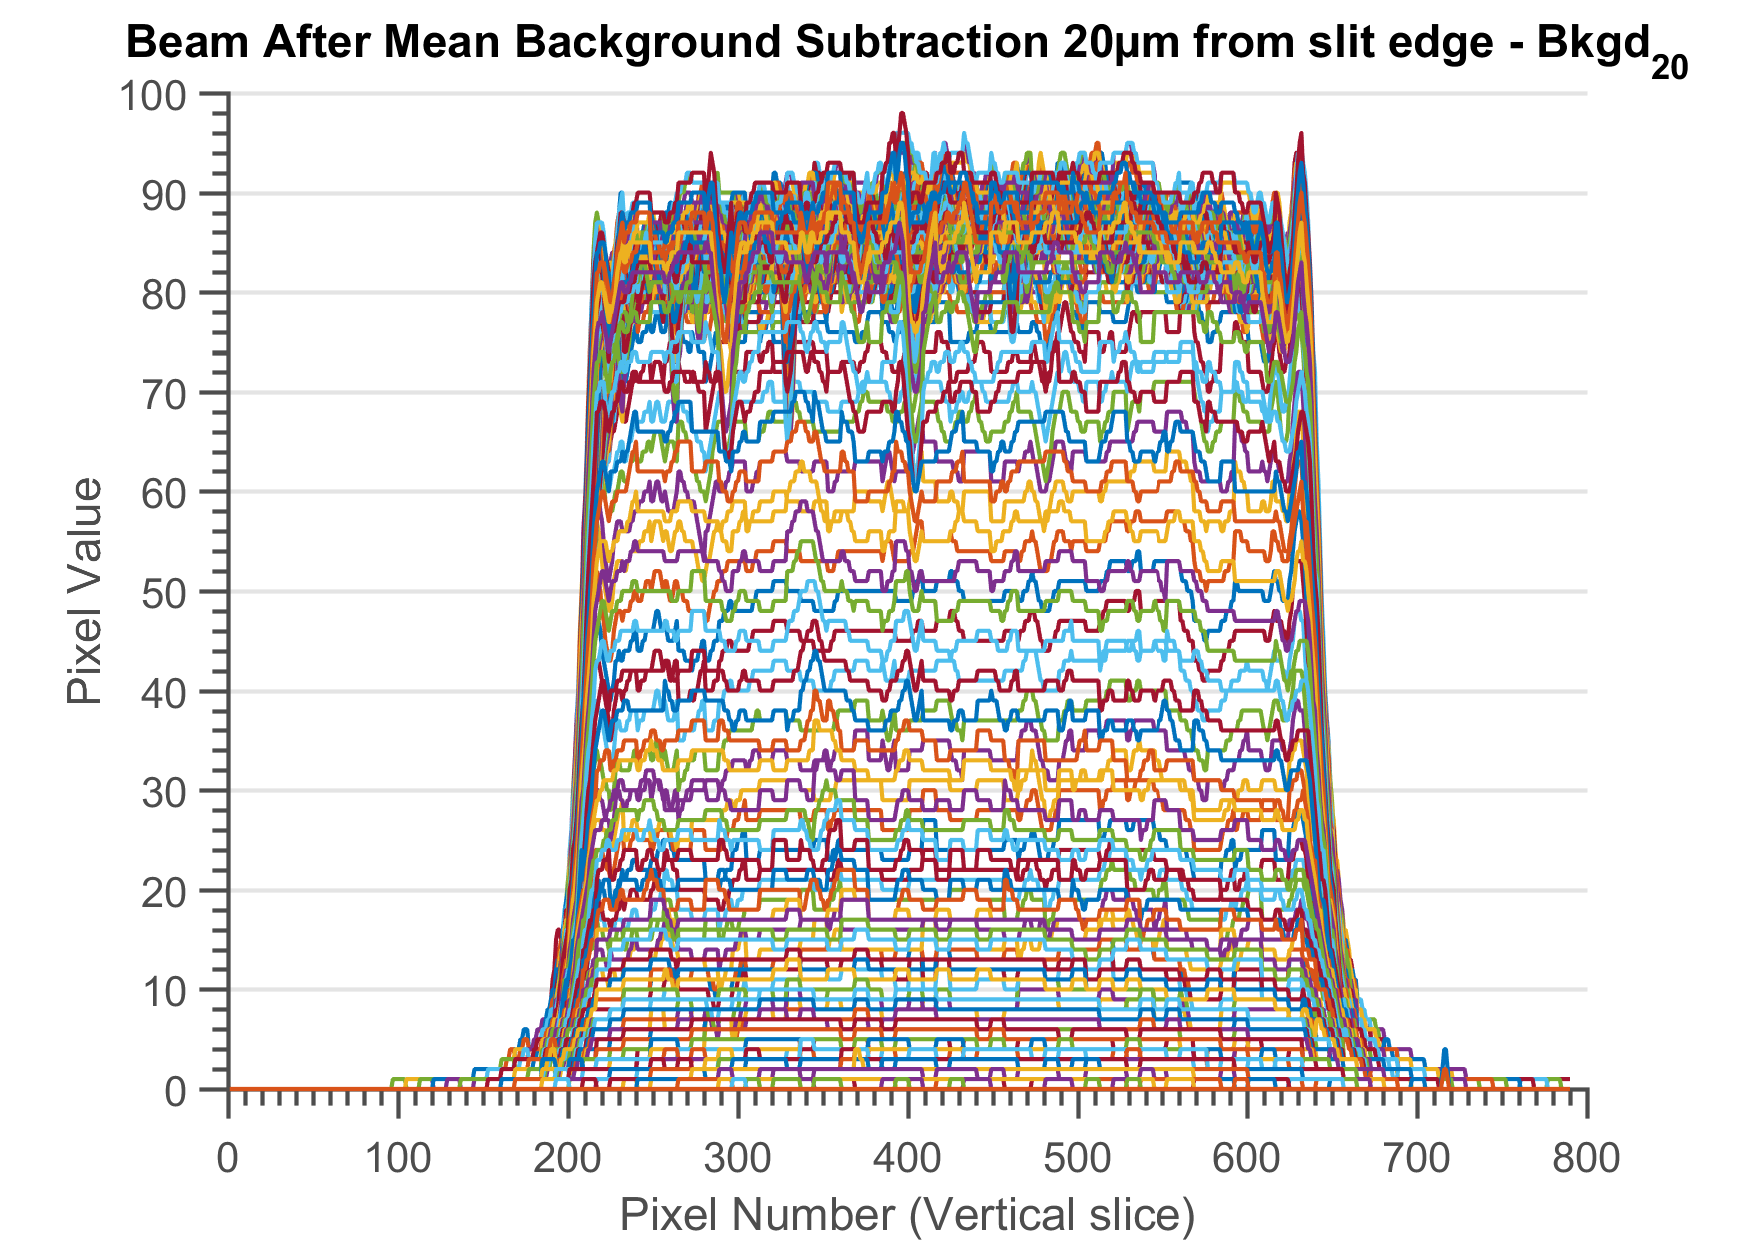
\includegraphics[width=\textwidth]{figures/beam/fig_beam_blind_thres160_mean.pdf}
                \caption{}
                \label{figallbeams6}
        \end{subfigure}
				\\
				\begin{subfigure}[b]{0.45\textwidth}
                \centering
                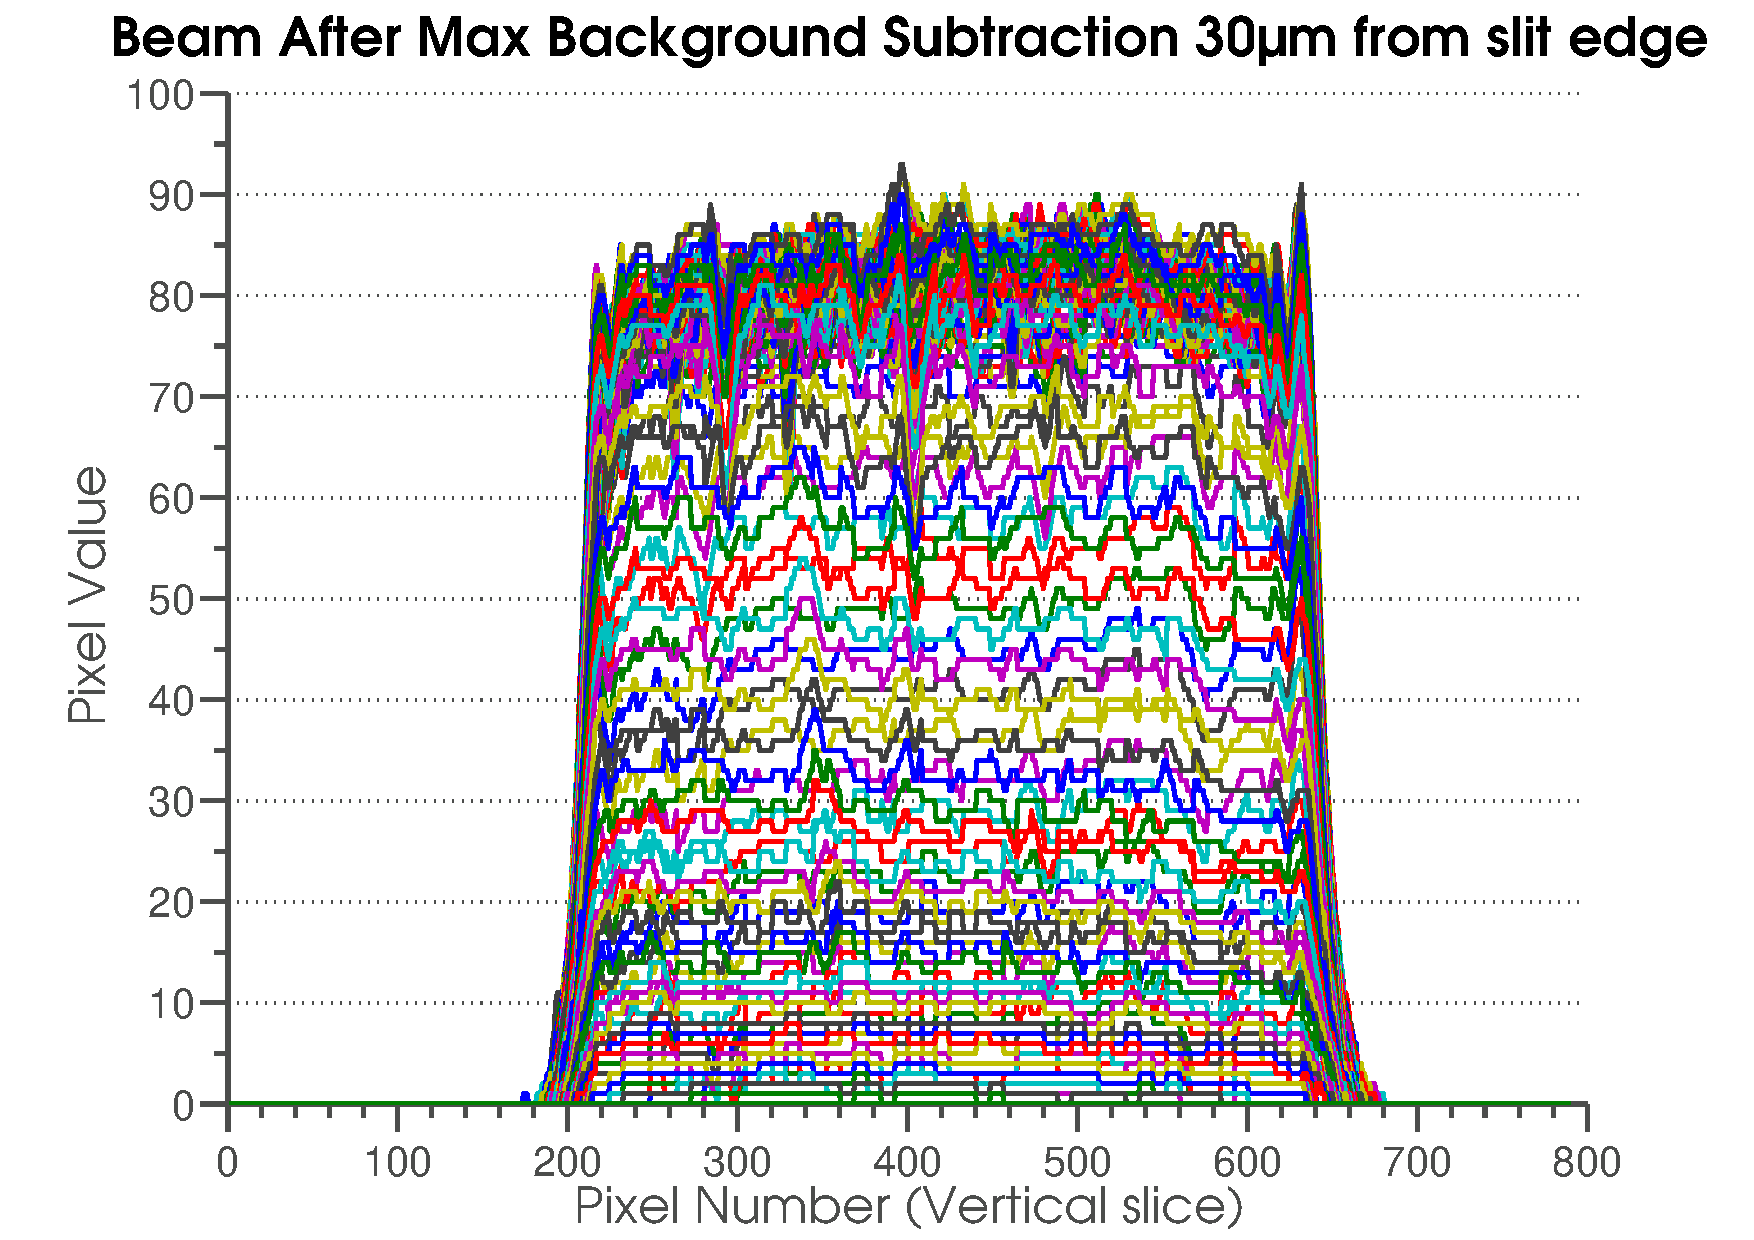
\includegraphics[width=\textwidth]{figures/beam/fig_beam_blind_thres170_max.pdf}
                \caption{}
                \label{figallbeams7}
        \end{subfigure}
				\qquad
        \begin{subfigure}[b]{0.45\textwidth}
                \centering
                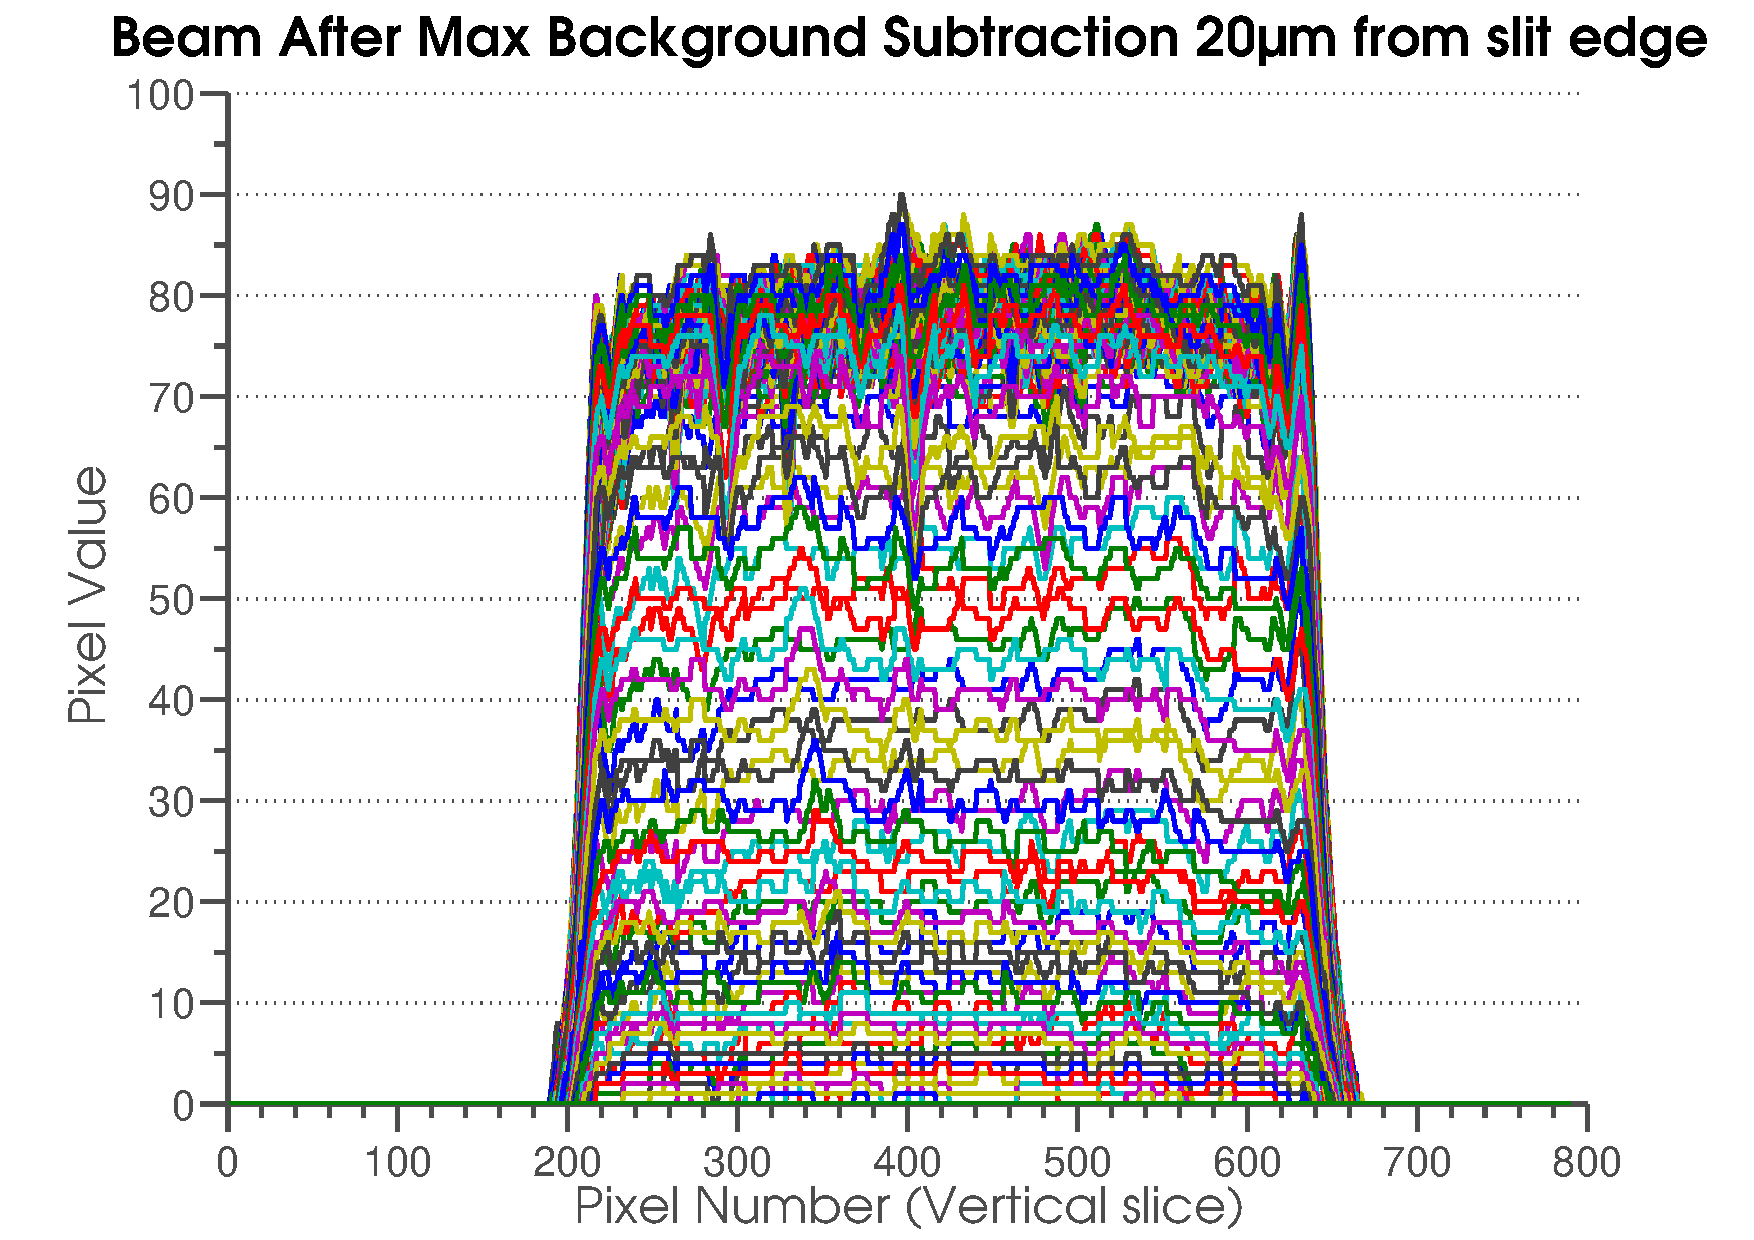
\includegraphics[width=\textwidth]{figures/beam/fig_beam_blind_thres160_max.pdf}
                \caption{}
                \label{figallbeams8}
        \end{subfigure}
		\label{figallbeams}
\end{figure}

\begin{figure}
\ContinuedFloat
	\centering
	\begin{subfigure}[b]{0.45\textwidth}
                \centering
                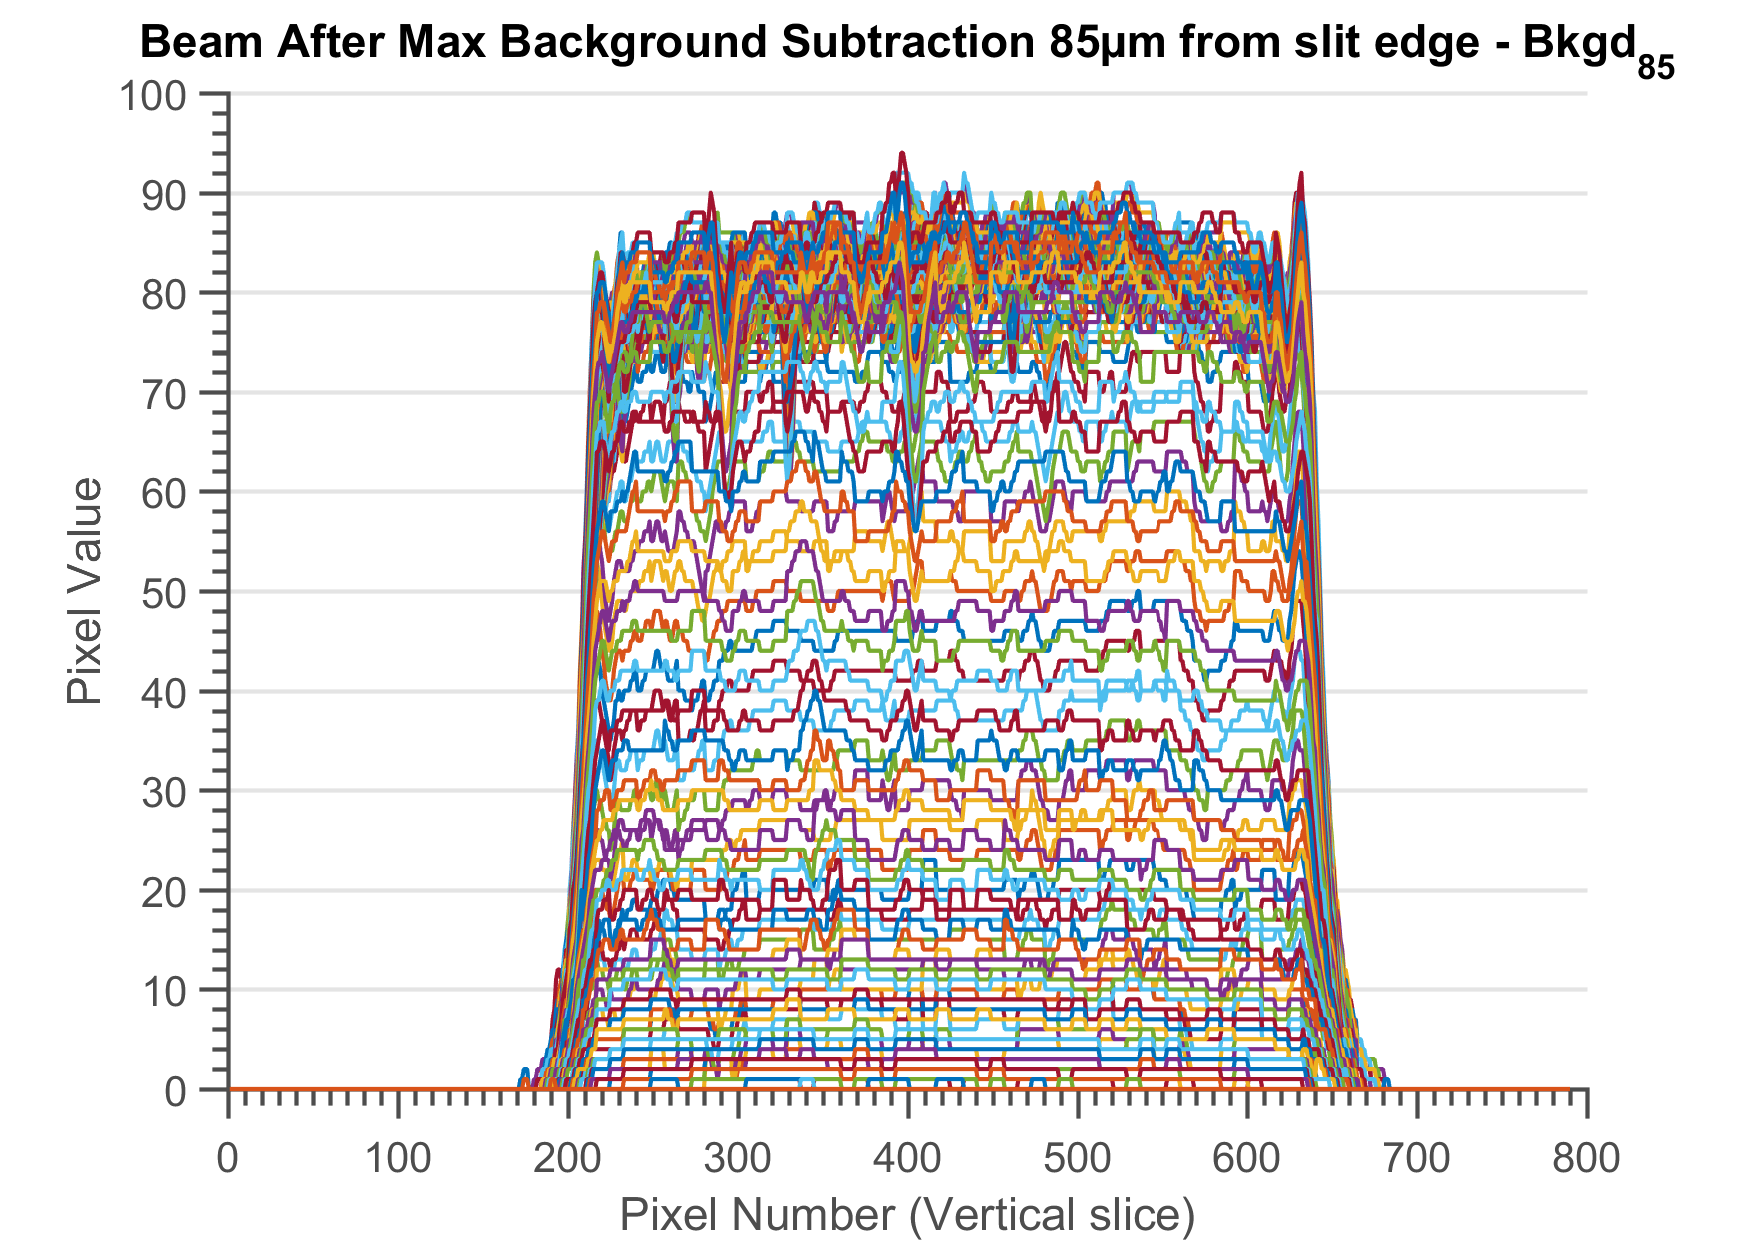
\includegraphics[width=\textwidth]{figures/beam/fig_beam_blind_thres225_max.pdf}
                \caption{}
                \label{figallbeams10}
        \end{subfigure}
				\qquad
        \begin{subfigure}[b]{0.45\textwidth}
                \centering
                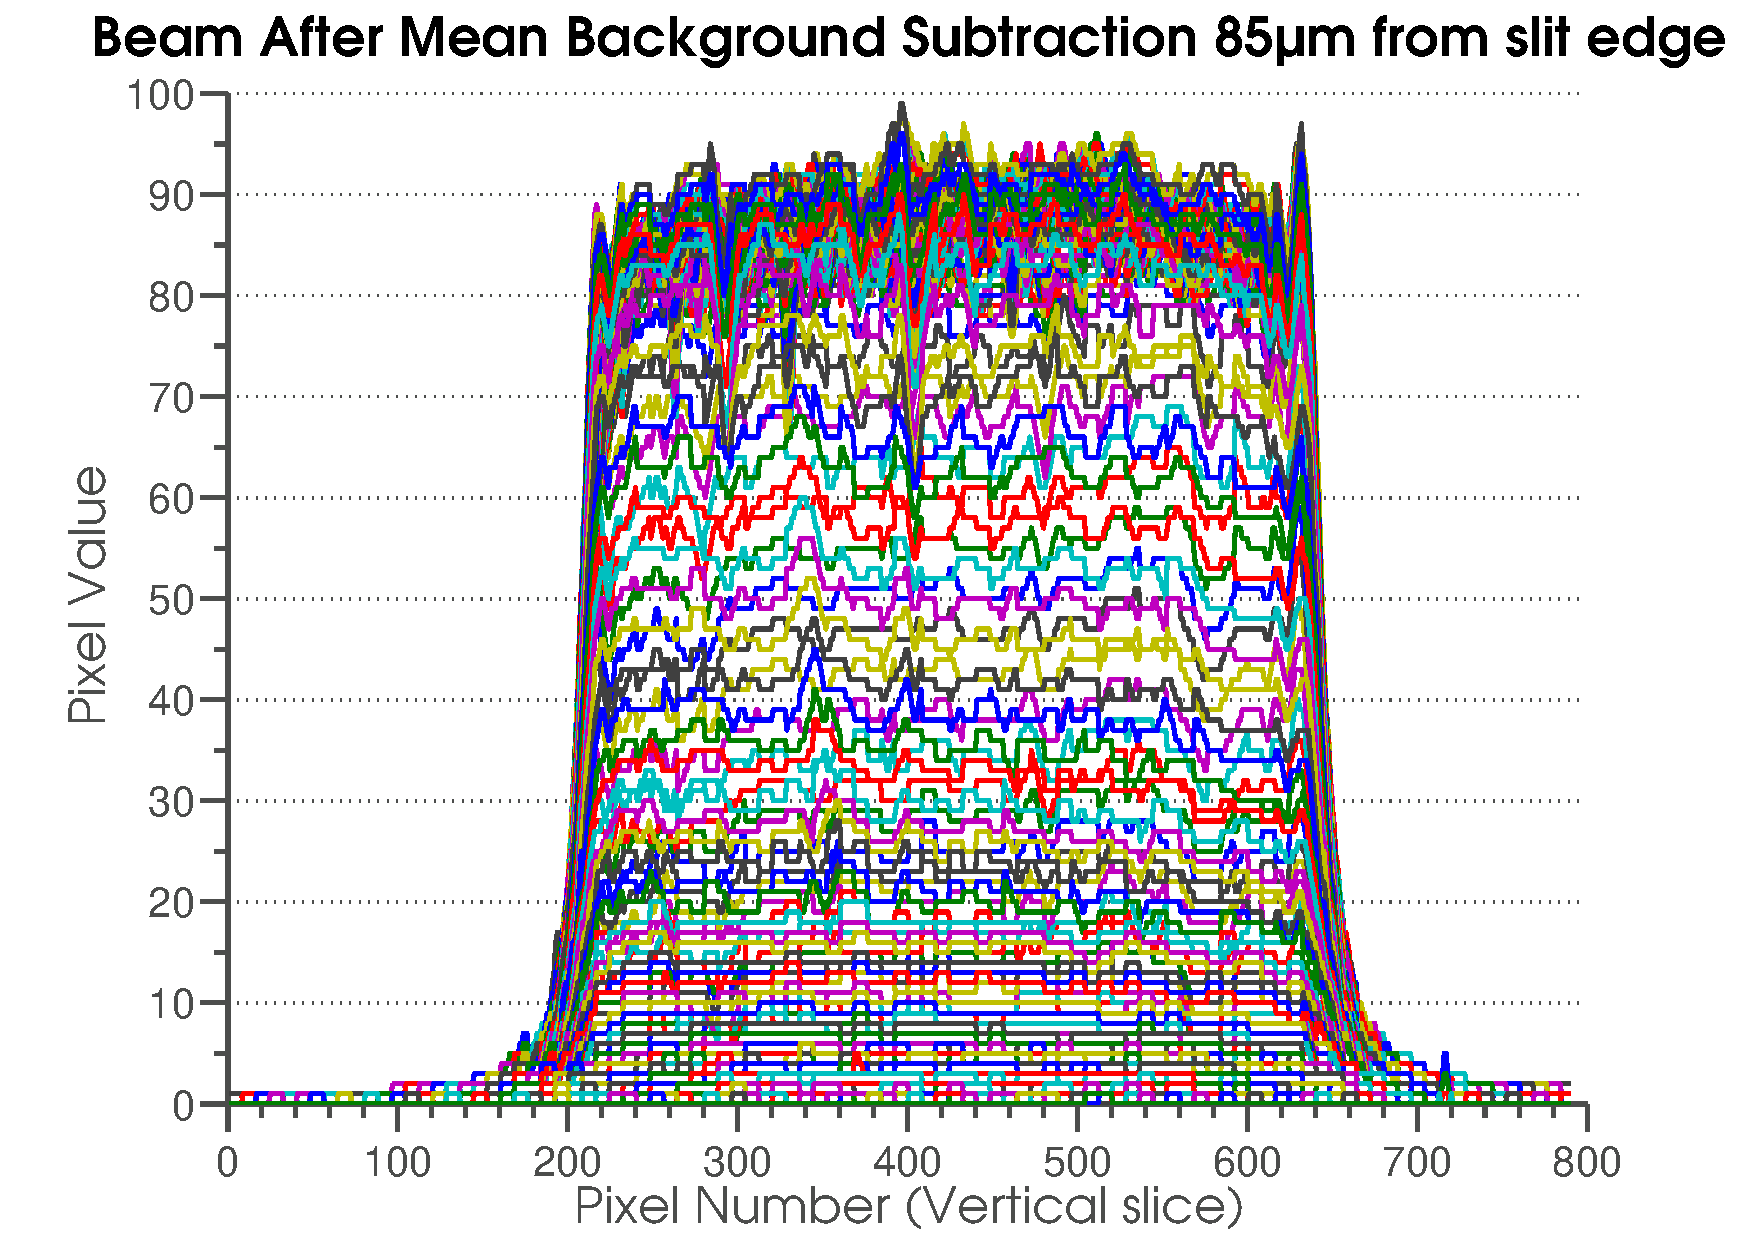
\includegraphics[width=\textwidth]{figures/beam/fig_beam_blind_thres225_mean.pdf}
                \caption{}
                \label{figallbeams11}
        \end{subfigure}
				\\
				\begin{subfigure}[b]{0.45\textwidth}
                \centering
                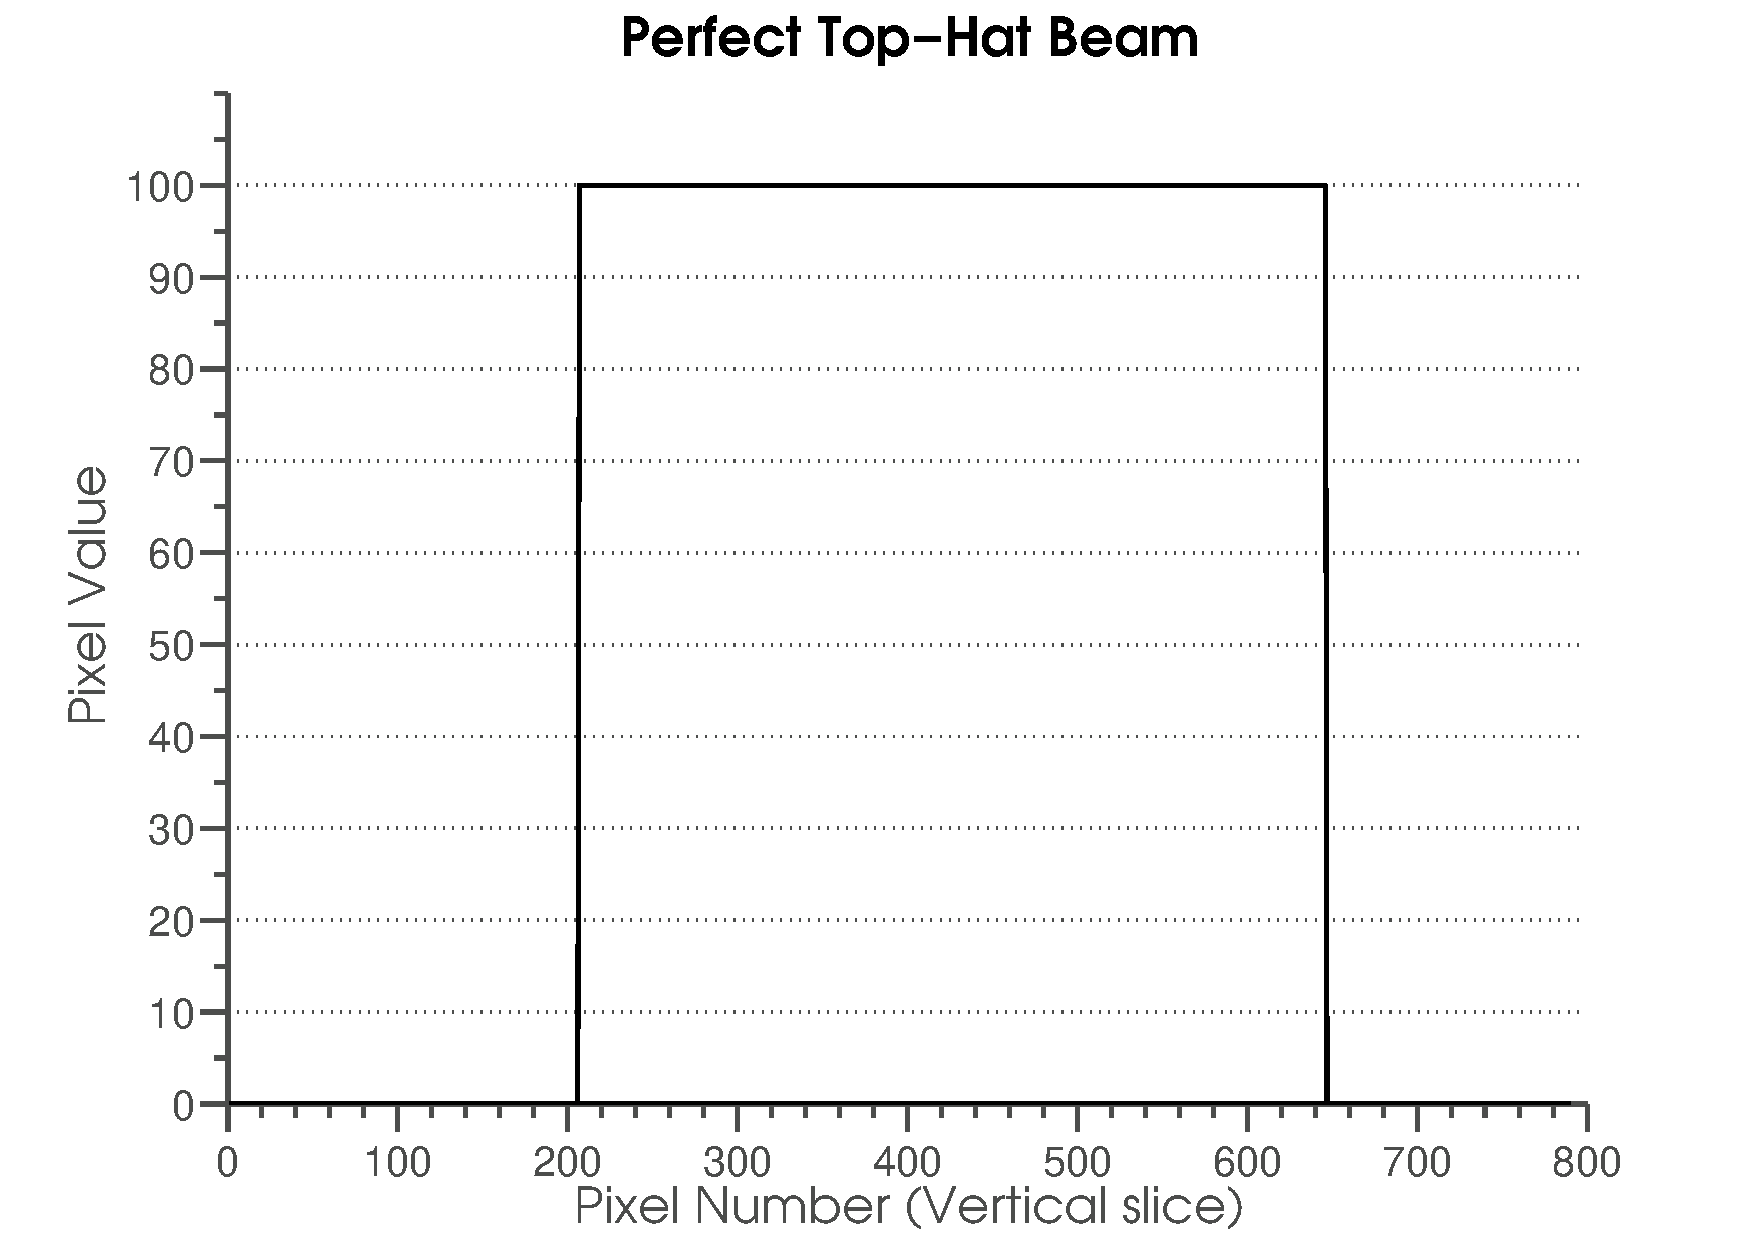
\includegraphics[width=\textwidth]{figures/beam/fig_beam_ideal.pdf}
                \caption{}
                \label{figallbeams9}
        \end{subfigure}
        \caption[Processed beam profiles used for simulations in RADDOSE-3D.]{Processed beam profiles used for simulations in RADDOSE-3D.
        Each figure is a plot with all vertical slices across the corresponding pgm images overlaid on a graph.
        They are essentially the same as Figure \ref{fig:Hamburg beamslice} except in these images all vertical slices are shown, as opposed to just the central slice.}
        \label{figallbeamscont}
\end{figure}

\subsection{RADDOSE-3D simulation results}
All of the beams illustrated in Figure~\ref{figallbeamscont} were used as input for RADDOSE-3D to simulate the experiment described in section \ref{sub:Data Collection and Dose Calculation} for insulin crystal ID 0259.
Each RADDOSE-3D run produced a set of DWD values; each value corresponded to one of the 271 datasets produced using the rolling window processing method described in section \ref{sub:Data Processing}.
These doses were plotted against the relative intensities ($I_n / I_1$) for each dataset and a line of best fit was determined using data where $I_n / I_1$ > 0.4.
$D_{1/2}$ values were then obtained from the line of best fit for each processed beam and plotted against the percentage of pixel values in the image that are equal to 0 as shown in Figure~\ref{figdhalf}.
The results show that the higher the threshold value (i.e. the more pixels that are considered background and are set to zero) the higher the $D_{1/2}$ value.
This occurs because RADDOSE-3D is run independently from the scaling of the diffraction data and therefore the $I_n/I_1$ values are the same for each run.
As alluded to above, more zero pixel values means that the same total photon flux is distributed over a smaller area (which always contained the crystal), and hence the crystal absorbs more energy which contributes to higher doses.
This gives the appearance that the crystal is less radiation sensitive (because the $D_{1/2}$ is higher).

The other major factor in the calculation of the dose values is the calculated absorption coefficients.
In Figure \ref{figdhalf} the blue markers correspond to simulations where the absorption coefficients were calculated with RADDOSE version 2 \cite{pait2009} (denoted RDV2 in Figure \ref{figdhalf}) giving an absorption coefficient of 4 $\times$ 10$^{\text{-4}}\, \mu m^{\text{-1}}$.
The red markers represent simulations where the absorption coefficients were calculated for an ``average protein'', H$_{\text{49.8}}$C$_{\text{31.8}}$N$_{\text{8.56}}$O$_{\text{9.54}}$S$_{\text{0.249}}$ (denoted \textit{``default''} in Figure \ref{figdhalf}).
The absorption coefficient assuming 50\% solvent is 2.37 $\times 10^{\text{-4}}\, \mu m^{\text{-1}}$ (details of the calculation can be found in \cite{holton2010}).
The absorption coefficient of insulin is bigger than that of the average protein because it contains more sulphur than the average protein, but it also contains zinc, which has a relatively high absorption cross section.
The difference between the absorption coefficients leads to differences in calculated doses of about a factor of 2.
\newline
The results seem to suggest that the two factors investigated here: beam profile and absorption coefficient, are the most important for dose calculations.
However, the differences between the profiles of the original beam image, the top hat beam and the deconvolved beam have a much less pronounced affect on the dose calculations compared to the absorption coefficient.
For example, the percentage difference of $D_{1/2}$ between the original beam with no background (denoted Original$_{\text{NB}}$ in the figure legend of Figure \ref{figdhalf}) and the deconvolved beam with no background is 0.8\% (using coefficients calculated using RADDOSE version 2).
This shows that deconvolution of the image will not significantly affect the dose estimate.
This is because the differences in the pixel values are relatively small when compared to the differences one may expect if a Gaussian beam profile is compared to a tophat profile.
\newline
Using the threshold method, there is a difference in $D_{1/2}$ ($\approx$ 3.9\% - 6.0\%) depending on the background threshold value) values if the maximum pixel value from the background is subtracted from the image or the mean pixel value is subtracted from the image.
This is consistent with the observation that the higher the threshold value, the higher the $D_{1/2}$ value.
The difference between the maximum threshold value from the 160 $\times$ 160$\, \mu m^2$ rectangle (Bkgd$_{\text{20}}$) and the mean value is 3.89\% (using RDV2 calculated absorption coefficients).
This result demonstrates that even if the area that is considered background is the same (Figure \ref{figbackgrounds}), deciding whether to subtract the mean background pixel value or the maximum pixel value will also have a small affect on the resulting $D_{1/2}$ value.

\begin{figure}
  \centering
    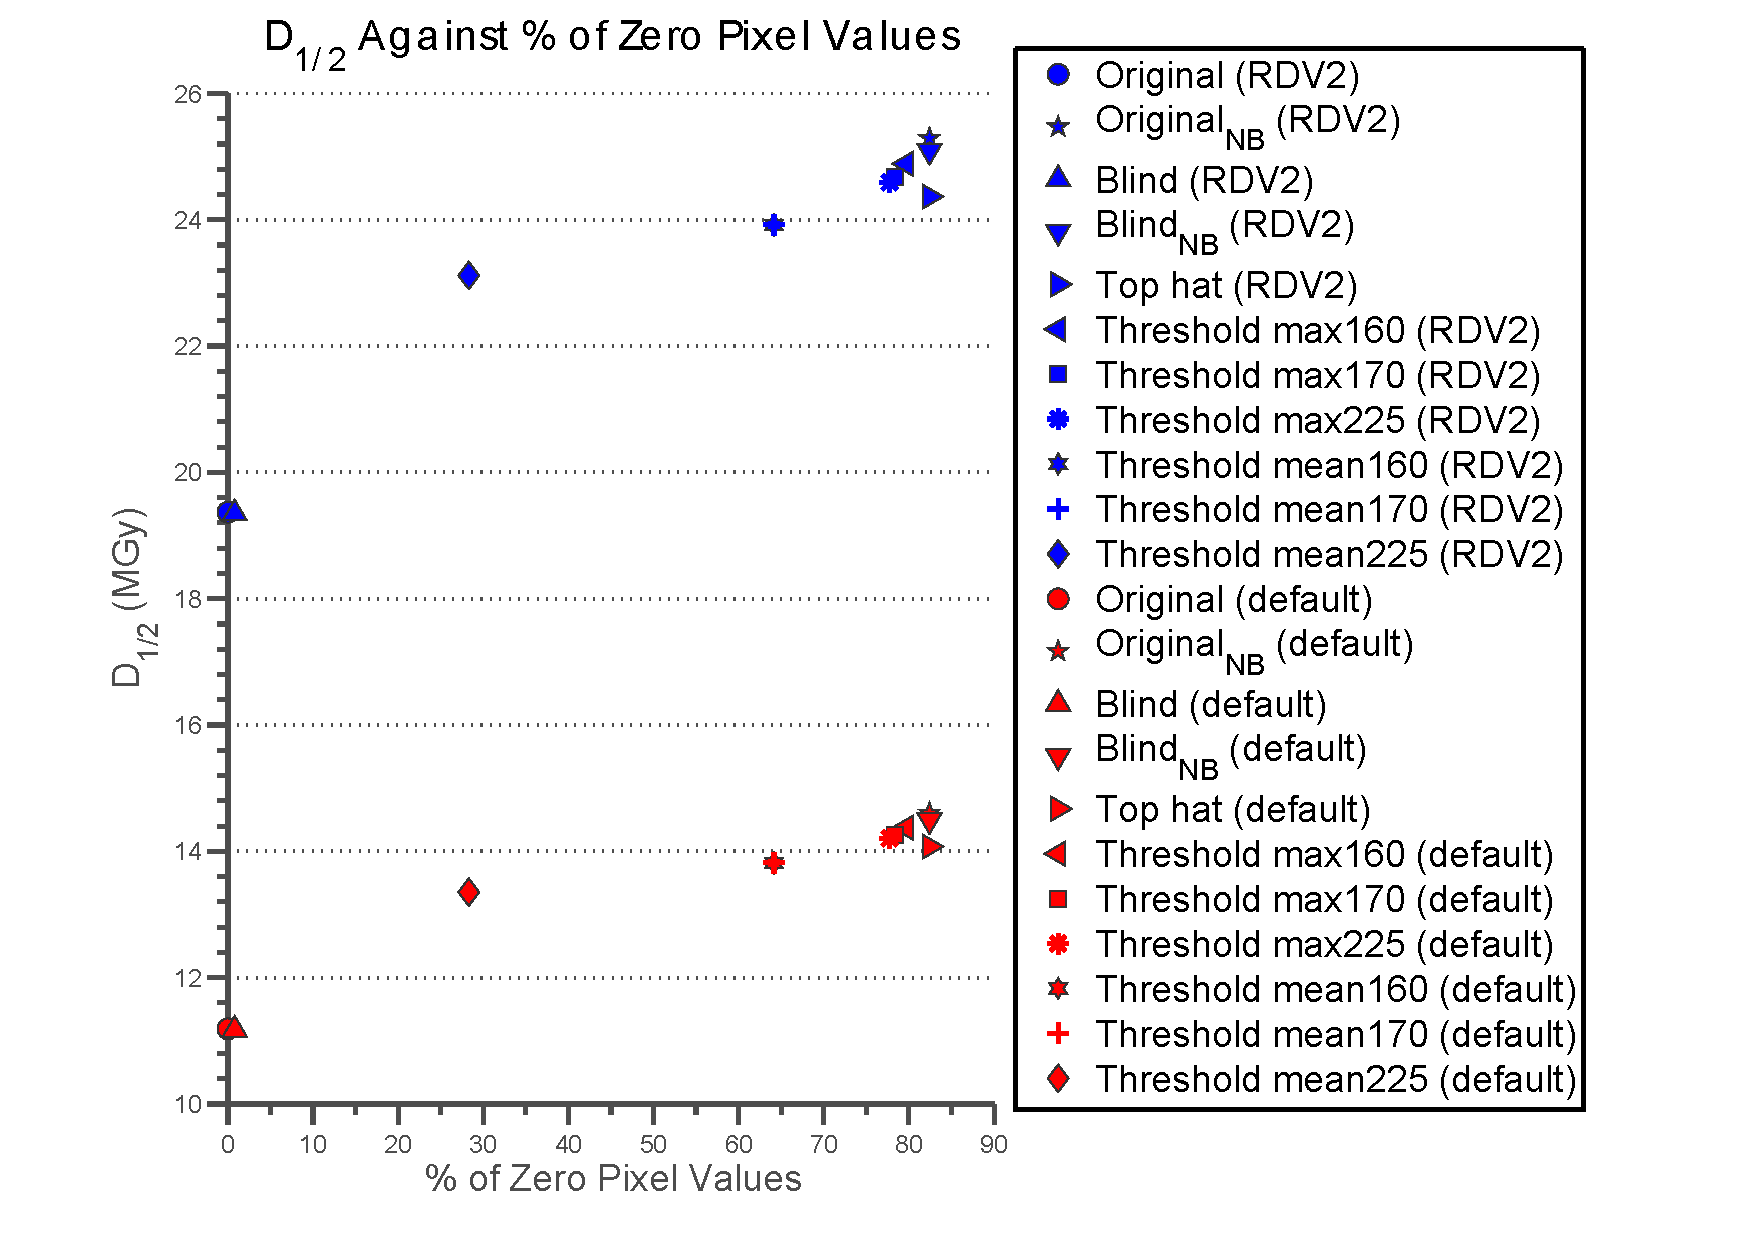
\includegraphics[width=1\textwidth]{figures/beam/d_half_plot.pdf}
    \caption[$D_{1/2}$ values plotted against the percentage of zero pixel values in the processed pgm beam images.]{$D_{1/2}$ values plotted against the percentage of zero pixel values in the processed pgm beam images.
    Blue markers correspond to simulations where the absorption coefficients were calculated with RADDOSE version 2 (denoted `RDV2' in figure legend) and red markers represent simulations where the absorption coefficients were calculated for an ``average protein'' (denoted `default' in figure legend).
    The subscript `NB' denotes beam profiles where the ``background'' was removed.
    The figure shows a trend that the higher the proportion of zero pixel values, the higher the $D_{1/2}$ value.
    It also shows that the method used to calculate the absorption coefficients can significantly affect the estimated doses.}
    \label{figdhalf}
\end{figure}
